
%%
%% forked from https://gits-15.sys.kth.se/giampi/kthlatex kthlatex-0.2rc4 on 2020-02-13
%% expanded upon by Gerald Q. Maguire Jr.
%% This template has been adapted by Anders Sjögren to the University
%% Engineering Program in Computer Science at KTH ICT. This adaptation was
%% translation of English headings into Swedish with the addition of Swedish.
%% Many thanks to others who have provided constructive input regarding the template.

% Make it possible to conditionally depend on the TeX engine used
\RequirePackage{ifxetex}
\RequirePackage{ifluatex}
\RequirePackage{etoolbox}
\newif\ifxeorlua
\ifxetex\xeorluatrue\fi
\ifluatex\xeorluatrue\fi

\ifxeorlua
% The following is to ensure that the PDF uses a recent version rather than the typical PDF 1-5
%  This same version of PDF should be set as an option for hyperef

\RequirePackage{expl3}


\ExplSyntaxOn
%pdf_version_gset:n{2.0}
%\pdf_version_gset:n{1.5}

%% Alternatively, if you have a LaTeX newer than June 2022, you can use the following. However, then you have to remove the pdfversion from hyperef. It also breaks hyperxmp. So perhaps it is too early to try using it!
%\DocumentMetadata
%{
%% testphase = phase-I, % tagging without paragraph tagging
% testphase = phase-II % tagging with paragraph tagging and other new stuff.
%pdfversion = 2.0 % pdfversion must be set here.
%}

% Optionally, you can set the uncompress flag to make it easier to examine the PDF
%\pdf_uncompress: % to check the pdf
\ExplSyntaxOff
\else
\RequirePackage{expl3}
\ExplSyntaxOn
%\pdf_version_gset:n{2.0}
\pdf_version_gset:n{1.5}
\ExplSyntaxOff
\fi

%% Define a pair of commands to disable and reenable specific packages - see https://tex.stackexchange.com/questions/39415/unload-a-latex-package
\makeatletter
\newcommand{\disablepackage}[2]{%
  \disable@package@load{#1}{#2}%
}
\newcommand{\reenablepackage}[1]{%
  \reenable@package@load{#1}%
}
\makeatother
%% To avoid the warning: "Package transparent Warning: Loading aborted, because pdfTeX is not running in PDF mode."
\ifxeorlua
\disablepackage{transparent}{}
\fi

%% The template is designed to handle a thesis in English or Swedish
\documentclass[english, bibtex]{kththesis}               % the bibliographic processor to use: biblatex or bibtex
%nomenclature,           % add the option nomenclature
%digitaloutput,          % optimize for digital output (this changes the color palette)
%includeExtraAbstracts, % uncomment to allow abstracts in languages beyond English & Swedish


% if pdflatex \usepackage[utf8]{inputenc}

%% Conventions for todo notes:
% Informational
%% \generalExpl{Comments/directions/... in English}
\newcommand*{\generalExpl}[1]{\todo[inline]{#1}}                

% Language-specific information (currently in English or Swedish)
\newcommand*{\engExpl}[1]{\todo[inline, backgroundcolor=kth-lightgreen40]{#1}} %% \engExpl{English descriptions about formatting}
\newcommand*{\sweExpl}[1]{\todo[inline, backgroundcolor=kth-lightblue40]{#1}}  %% % \sweExpl{Text på svenska}

% warnings
\newcommand*{\warningExpl}[1]{\todo[inline, backgroundcolor=kth-lightred40]{#1}} %% \warningExpl{warnings}

% Hide all template todo notes for the final compile.
\renewcommand\warningExpl[1]{}
\renewcommand\generalExpl[1]{}
\renewcommand\engExpl[1]{}
\renewcommand\sweExpl[1]{}


% \usepackage[style=numeric,sorting=none,backend=biber]{biblatex}
\iftoggle{biblatex}{
    %\usepackage[language=english,bibstyle=authoryear,citestyle=authoryear, maxbibnames=99]{biblatex}
    % Alternatively you might use another style, such as IEEE and use citestyle=numeric-comp  to put multiple citations in a single pair of square brackets
    \usepackage[style=ieee,citestyle=numeric-comp]{biblatex}
    \addbibresource{references.bib}
    %\DeclareLanguageMapping{norsk}{norwegian}
}{
    % The line(s) below are for BibTeX
    \bibliographystyle{bibstyle/myIEEEtran}
    %\bibliographystyle{apalike}
}


% include a variety of packages that are useful
\input{lib/includes}
\input{lib/kthcolors}

%\glsdisablehyper
%\makeglossaries
%\makenoidxglossaries
%%%% Local Variables:
%%% mode: latex
%%% TeX-master: t
%%% End:
% The following command is used with glossaries-extra
\setabbreviationstyle[acronym]{long-short}
% The form of the entries in this file is \newacronym{label}{acronym}{phrase}
%                                      or \newacronym[options]{label}{acronym}{phrase}

\newacronym{auprc}{AUPRC}{area under the precision-recall curve}
\newacronym{auroc}{AUROC}{area under the receiver operating characteristic curve}
\newacronym{cpu}{CPU}{central processing unit}
\newacronym{json}{JSON}{JavaScript Object Notation}
\newacronym{API}{API}{application programming interface}
\newacronym{bert}{BERT}{Bidirectional Encoder Representations from Transformers}
\newacronym{gpu}{GPU}{graphics processing unit}
\newacronym[longplural={large language models}]{llm}{LLM}{large language model}
\newacronym{llmjudge}{LLM-as-a-Judge}{large language model as a judge}
\newacronym{qa}{QA}{question answering}
\newacronym{rag}{RAG}{Retrieval-Augmented Generation}
\newacronym{tfidf}{TF-IDF}{term frequency-inverse document frequency}
\newacronym{UN}{UN}{United Nations}
\newacronym{SDG}{SDG}{Sustainable Development Goal}
                %load the acronyms file

\input{lib/defines}  % load some additional definitions to make writing more consistent

% The following is needed in conjunction with generating the DiVA data with abstracts and keywords using the scontents package and a modified listings environment
%\usepackage{listings}   %  already included

\makeatletter
\let\verbatimsc\@undefined
\let\endverbatimsc\@undefined
\lst@AddToHook{Init}{\hyphenpenalty=50\relax}
\makeatother


\lstnewenvironment{verbatimsc}
    {
    \lstset{%
        basicstyle=\ttfamily\tiny,
        backgroundcolor=\color{white},
        %basicstyle=\tiny,
        %columns=fullflexible,
        columns=[l]fixed,
        language=[LaTeX]TeX,
        %numbers=left,
        %numberstyle=\tiny\color{gray},
        keywordstyle=\color{red},
        breaklines=true,                 % sets automatic line breaking
        breakatwhitespace=true,          % sets if automatic breaks should only happen at whitespace
        %keepspaces=false,
        breakindent=0em,
        %fancyvrb=true,
        frame=none,                     % turn off any box
        postbreak={}                    % turn off any hook arrow for continuation lines
    }
}{}

%% Add some more keywords to bring out the structure more
\lstdefinestyle{[LaTeX]TeX}{
morekeywords={begin, todo, textbf, textit, texttt}
}

%% definition of new command for bytefield package
\newcommand{\colorbitbox}[3]{%
	\rlap{\bitbox{#2}{\color{#1}\rule{\width}{\height}}}%
	\bitbox{#2}{#3}}




% define a left aligned table cell that is ragged right
\newcolumntype{L}[1]{>{\raggedright\let\newline\\\arraybackslash\hspace{0pt}}p{#1}}

% Because backref is not compatible with biblatex
\iftoggle{biblatex}{
    \usepackage[plainpages=false]{hyperref}
}{
    \usepackage[
    backref=page,
    pagebackref=false,
    plainpages=false,
                            % PDF related options
    unicode=true,           % Unicode encoded PDF strings
    bookmarks=true,         % generate bookmarks in PDF files
    bookmarksopen=false,    % Do not automatically open the bookmarks in the PDF reading program
    pdfpagemode=UseNone,    % None, UseOutlines, UseThumbs, or FullScreen
    destlabel,              % better naming of destinations
    pdfencoding=auto,       % for unicode in 
    ]{hyperref}
   %% Removed use of backref package as it is incompatible with using attachfile
}

\usepackage[all]{hypcap}	%% prevents an issue related to hyperref and caption linking

%% Acronyms
% note that nonumberlist - removes the cross references to the pages where the acronym appears
% note that super will set the descriptions text aligned
% note that nomain - does not produce a main glossary, thus only acronyms will be in the glossary
% note that nopostdot - will prevent there being a period at the end of each entry
\usepackage[acronym, style=super, section=section, nonumberlist, nomain,
nopostdot]{glossaries}
\setlength{\glsdescwidth}{0.75\textwidth}
\usepackage[]{glossaries-extra}
\ifinswedish
    %\usepackage{glossaries-swedish}
\fi

%% For use with the README_notes
% Define a new type of glossary so that the acronyms defined in the README_notes document can be distinct from those in the thesis template
% the tlg, tld, and dn will be the file extensions used for this glossary
\newglossary[tlg]{readme}{tld}{tdn}{README acronyms}


\input{lib/includes-after-hyperref}

%\glsdisablehyper
\makeglossaries
%\makenoidxglossaries

% The following bit of ugliness is because of the problems PDFLaTeX has handling a non-breaking hyphen
% unless it is converted to UTF-8 encoding.
% If you do not use such characters in your acronyms, this could be simplified to just include the acronyms file.
\ifxeorlua
%%% Local Variables:
%%% mode: latex
%%% TeX-master: t
%%% End:
% The following command is used with glossaries-extra
\setabbreviationstyle[acronym]{long-short}
% The form of the entries in this file is \newacronym{label}{acronym}{phrase}
%                                      or \newacronym[options]{label}{acronym}{phrase}

\newacronym{auprc}{AUPRC}{area under the precision-recall curve}
\newacronym{auroc}{AUROC}{area under the receiver operating characteristic curve}
\newacronym{cpu}{CPU}{central processing unit}
\newacronym{json}{JSON}{JavaScript Object Notation}
\newacronym{API}{API}{application programming interface}
\newacronym{bert}{BERT}{Bidirectional Encoder Representations from Transformers}
\newacronym{gpu}{GPU}{graphics processing unit}
\newacronym[longplural={large language models}]{llm}{LLM}{large language model}
\newacronym{llmjudge}{LLM-as-a-Judge}{large language model as a judge}
\newacronym{qa}{QA}{question answering}
\newacronym{rag}{RAG}{Retrieval-Augmented Generation}
\newacronym{tfidf}{TF-IDF}{term frequency-inverse document frequency}
\newacronym{UN}{UN}{United Nations}
\newacronym{SDG}{SDG}{Sustainable Development Goal}
                %load the acronyms file
\else
\input{lib/acronyms-for-pdflatex}
\fi

% place holders for languages lacking .lbx files
\input{lib/placeHolder_lbx_files}

% insert the configuration information with author(s), examiner, supervisor(s), ...
\input{custom_configuration}

% read in the plain text definitions, if they exist
\IfFileExists{custom_configuration_plaintext.tex}{\input{custom_configuration_plaintext.tex}}{}


% Enter the English and Swedish keywords here for use in the PDF metadata _and_ for later use
% following the respective abstract.
% Try to put the words in the same order in both languages to facilitate matching. For example:
\EnglishKeywords{Retrieval-Augmented Generation, Hybrid RAG, Query routing, ModernBERT, 2WikiMultihopQA, LLM-as-a-Judge, Routing-label classification, Routed cost}
\SwedishKeywords{Retrieval-Augmented Generation, hybrid-RAG, frågeroutning, ModernBERT, 2WikiMultihopQA, LLM-som-domare, routingklassificering, routad kostnad}

%%%%% For the oral presentation
%% Add this information once your examiner has scheduled your oral presentation
\presentationDateAndTimeISO{}
\presentationLanguage{}  % generally: eng or swe
\presentationRoom{}
\presentationAddress{}
\presentationCity{Stockholm}

% When there are multiple opponents, separate their names with '\&'
% Opponent's information
%\opponentsNames{A. B. Normal \& A. X. E. Normalè}
\opponentsNames{}

% It is possible to have a cover illustration
%\coverIllustration{figures/image1.png}
% if so, the author might acknowledge this or give the copyright information for it with:
%\coverIllustrationCredit{A. B. Normal}

% Once a thesis is approved by the examiner, add the TRITA number
% The TRITA number for a thesis consists of two parts: a series (unique to each school)
% and the number in the series, which is formatted as the year followed by a colon and
% then a unique series number for the thesis - starting with 1 each year.
%\trita{TRITA -- XXX-EX}{2026:0000}

% Put the title, author, and keyword information into the PDF meta information
\input{lib/pdf_related_includes}


% the custom colors and the commands are defined in defines.tex    
\hypersetup{
	colorlinks  = true,
	breaklinks  = true,
	linkcolor   = \linkscolor,
	urlcolor    = \urlscolor,
	citecolor   = \refscolor,
	anchorcolor = black
}

\ifnomenclature
% The following lines make the page numbers and equations hyperlinks in the Nomenclature list
\renewcommand*{\pagedeclaration}[1]{\unskip, \dotfill\hyperlink{page.#1}{page\nobreakspace#1}}
% The following does not work correctly, as the name of the cross-reference is incorrect
%\renewcommand*{\eqdeclaration}[1]{, see equation\nobreakspace(\hyperlink{equation.#1}{#1})}

% You can also change the page heading for the nomenclature
\renewcommand{\nomname}{List of Symbols Used}

% You can even add customization text before the list
\renewcommand{\nompreamble}{The following symbols will be later used within the body of the thesis.}
\makenomenclature
\fi

%
% The commands below are to configure JSON listings
% 
% format for JSON listings
\colorlet{punct}{red!60!black}
\definecolor{delim}{RGB}{20,105,176}
\definecolor{numb}{RGB}{106, 109, 32}
\definecolor{string}{RGB}{0, 0, 0}

\lstdefinelanguage{json}{
    numbers=none,
    numberstyle=\small,
    frame=none,
    rulecolor=\color{black},
    showspaces=false,
    showtabs=false,
    breaklines=true,
    postbreak=\raisebox{0ex}[0ex][0ex]{\ensuremath{\color{gray}\hookrightarrow\space}},
    breakatwhitespace=true,
    basicstyle=\ttfamily\small,
    extendedchars=false,
    upquote=true,
    morestring=[b]",
    stringstyle=\color{string},
    literate=
     *{0}{{{\color{numb}0}}}{1}
      {1}{{{\color{numb}1}}}{1}
      {2}{{{\color{numb}2}}}{1}
      {3}{{{\color{numb}3}}}{1}
      {4}{{{\color{numb}4}}}{1}
      {5}{{{\color{numb}5}}}{1}
      {6}{{{\color{numb}6}}}{1}
      {7}{{{\color{numb}7}}}{1}
      {8}{{{\color{numb}8}}}{1}
      {9}{{{\color{numb}9}}}{1}
      {:}{{{\color{punct}{:}}}}{1}
      {,}{{{\color{punct}{,}}}}{1}
      {\{}{{{\color{delim}{\{}}}}{1}
      {\}}{{{\color{delim}{\}}}}}{1}
      {[}{{{\color{delim}{[}}}}{1}
      {]}{{{\color{delim}{]}}}}{1}
      {’}{{\char13}}1,
}

\lstdefinelanguage{XML}
{
  basicstyle=\ttfamily\color{blue}\bfseries\small,
  morestring=[b]",
  morestring=[s]{>}{<},
  morecomment=[s]{<?}{?>},
  stringstyle=\color{black},
  identifierstyle=\color{blue},
  keywordstyle=\color{cyan},
  breaklines=true,
  postbreak=\raisebox{0ex}[0ex][0ex]{\ensuremath{\color{gray}\hookrightarrow\space}},
  breakatwhitespace=true,
  morekeywords={xmlns,version,type}% list your attributes here
}

% If you use both listing and lstlisting environments - the following makes them both use the same counter and the same formatting in the List of Listings
\makeatletter
\AtBeginDocument{\let\c@listing\c@lstlisting}
\AtBeginDocument{\let\l@listing\l@lstlisting}
\makeatother

% Change the heading for the "List of Listings" to simply "Listings"
\renewcommand{\lstlistlistingname}{Listings}

% number each listing within the chapter
\numberwithin{listing}{chapter}

\usepackage{subfiles}

% To have Creative Commons (CC) license and logos use the doclicense package
% Note that the lowercase version of the license has to be used in the modifier
% i.e., one of by, by-nc, by-nd, by-nc-nd, by-sa, by-nc-sa, zero.
% For background see:
% https://www.kb.se/samverkan-och-utveckling/oppen-tillgang-och-bibsamkonsortiet/open-access-and-bibsam-consortium/open-access/creative-commons-faq-for-researchers.html
% https://kib.ki.se/en/publish-analyse/publish-your-article-open-access/open-licence-your-publication-cc
\begin{comment}
\usepackage[
    type={CC},
    %modifier={by-nc-nd},
    %version={4.0},
    modifier={by-nc},
    imagemodifier={-eu-88x31},  % to get Euro symbol rather than Dollar sign
    hyphenation={RaggedRight},
    version={4.0},
    %modifier={zero},
    %version={1.0},
]{doclicense}
\end{comment}
\listfiles

\begin{document}
%\selectlanguage{swedish}
%
\selectlanguage{english}

%%% Set the numbering for the title page to a numbering series not in the preface or body
\pagenumbering{alph}
\kthcover
\clearpage\thispagestyle{empty}\mbox{} % empty back of front cover
\titlepage

% If you do not want to have a bookinfo page, comment out the line saying \bookinfopage and add a \cleardoublepage
% If you want a bookinfo page: you will get a copyright notice, unless you have used the doclicense package in which case you will get a Creative Commons license. To include the doclicense package, uncomment the configuration of this package above and configure it with your choice of license.
\bookinfopage

% Frontmatter includes the abstracts and table-of-contents
\frontmatter
\setcounter{page}{1}
\begin{abstract}
% The first abstract should be in the language of the thesis.
% Abstract fungerar på svenska också.
  \markboth{\abstractname}{}
\begin{scontents}[store-env=lang]
eng
\end{scontents}
%%% The contents of the abstract (between the begin and end of scontents) will be saved in LaTeX format
%%% and output on the page(s) at the end of the thesis with information for DiVA facilitating the correct
%%% entry of the meta data for your thesis.
%%% These page(s) will be removed before the thesis is inserted into DiVA.
\engExpl{All theses at KTH are \textbf{required} to have an abstract in both \textit{English} and \textit{Swedish}.}

\engExpl{Exchange students may want to include one or more abstracts in the language(s) used in their home institutions to avoid the need to write another thesis when returning to their home institution.}

\generalExpl{Keep in mind that most of your potential readers are only going to read your \texttt{title} and \texttt{abstract}. This is why the abstract must give them enough information so that they can decide if this document is relevant to them or not. Otherwise, the likely default choice is to ignore the rest of your document.\\
An abstract should stand on its own, \ie no citations, cross-references to the body of the document, acronyms must be spelled out, \ldots .\\Write this early and revise as necessary. This will help keep you focused on what you are trying to do.}

\begin{scontents}[store-env=abstracts,print-env=true]
Retrieval-Augmented Generation (RAG) is a common approach for grounding large language models in external knowledge. Production systems increasingly combine cheap vector retrieval with more expensive graph-enhanced retrieval, because graph-enhanced retrieval can help answer questions whose evidence is split across documents but uses substantially more compute than vector retrieval. Applying graph-enhanced retrieval to every query wastes resources on questions that the cheap path could already handle, while always using vector retrieval risks missing questions that benefit from the richer retrieval mode.

This thesis studies whether the choice between a cheap vector retrieval mode and a more expensive graph-enhanced retrieval mode can be predicted from the query text alone. The setting is the 2WikiMultihopQA benchmark inside the LightRAG retrieval framework, with LightRAG's Naive mode as the cheap path and its Mix mode as the graph-enhanced path. Routing labels are constructed by running both retrieval modes on every benchmark question and using a large language model as a judge to compare each mode's answer against the gold answer. The resulting binary routing dataset is split jointly by question type and routing label, and is used to train and evaluate two query-only routers: a TF-IDF logistic-regression baseline and a fine-tuned ModernBERT classifier.

On a held-out test split of 193 queries, the ModernBERT router achieves higher point estimates than the TF-IDF baseline on aggregate routing-label classification metrics, including area under the precision-recall curve (0.769 vs.\ 0.742), balanced routing-label accuracy (0.798 vs.\ 0.784), and F1 on the minority class (0.699 vs.\ 0.650), with differences that are stable across three training seeds. The ModernBERT router also improves over a non-deployable diagnostic heuristic that routes by a coarse question-category label, while needing only the query text as input. Treated as offline routing policies and evaluated along two routed-cost dimensions, both learned routers route at substantially lower mean cost than always using the Mix mode. The ModernBERT router reduces mean routed execution time by 39\,\% and estimated mean routed model-token usage by 60\,\% relative to the always-Mix baseline. Mean token usage is estimated from per-mode means measured on an instrumented subset of \(N = 150\) queries spanning all four 2WikiMultihopQA question types. These metrics evaluate whether the router selects the judge-derived minimum sufficient retrieval mode, not an independently re-judged final answer accuracy of the routed system. Within this experimental setting, the retrieval-mode distinction is partly predictable from the query text alone, and a lightweight encoder classifier is a promising routing layer for adaptive Hybrid RAG.
\end{scontents}

\subsection*{Keywords}
\begin{scontents}[store-env=keywords,print-env=true]
% If you set the EnglishKeywords earlier, you can retrieve them with:
\InsertKeywords{english}
% If you did not set the EnglishKeywords earlier then simply enter the keywords here:
% comma separate keywords, such as: Canvas Learning Management System, Docker containers, Performance tuning
\end{scontents}
\end{abstract}
\cleardoublepage
\babelpolyLangStart{swedish}
\begin{abstract}
    \markboth{\abstractname}{}
\begin{scontents}[store-env=lang]
swe
\end{scontents}
\warningExpl{Inside the following scontents environment, you cannot use a \textbackslash include{filename} as the command rather than the file contents will end up in the for DiVA information. Additionally, you should not use a straight double quote character in the abstracts or keywords, use two single quote characters instead.}
\sweExpl{Alla avhandlingar vid KTH \textbf{måste ha} ett abstrakt på både \textit{engelska} och \textit{svenska}.\\
Om du skriver din avhandling på svenska ska detta göras först (och placera det som det första abstraktet) - och du bör revidera det vid behov.}

\engExpl{If you are writing your thesis in English, you can leave this until the draft version that goes to your opponent for the written opposition. In this way, you can provide the English and Swedish abstract/summary information that can be used in the announcement for your oral presentation.\\If you are writing your thesis in English, then this section can be a summary targeted at a more general reader. However, if you are writing your thesis in Swedish, then the reverse is true – your abstract should be for your target audience, while an English summary can be written targeted at a more general audience.\\This means that the English abstract and Swedish sammnfattning  
or Swedish abstract and English summary need not be literal translations of each other.}

\warningExpl{Do not use the \textbackslash glspl\{\} command in an abstract that is not in English, as my programs do not know how to generate plurals in other languages. Instead, you will need to spell these terms out or give the proper plural form. In fact, it is a good idea not to use the glossary commands at all in an abstract/summary in a language other than the language used in the \texttt{acronyms.tex file} - since the glossary package does \textbf{not} support use of more than one language.}

\engExpl{The abstract in the language used for the thesis should be the first abstract, while the Summary/Sammanfattning in the other language can follow}
\begin{scontents}[store-env=abstracts,print-env=true]
Retrieval-Augmented Generation (RAG) är en vanlig arkitektur för att förankra stora språkmodeller i externt material. I moderna system kombineras allt oftare billig vektorbaserad sökning med dyrare grafbaserad hämtning, eftersom grafbaserad hämtning kan hjälpa till att besvara frågor vars belägg är fördelade över flera dokument men kräver väsentligt mer beräkningsresurser än vektorbaserad sökning. Att tillämpa den grafbaserade hämtningen på varje fråga slösar resurser på frågor som den billigare metoden redan klarar, medan att alltid använda enbart vektorsökning riskerar att missa frågor som drar nytta av det mer omfattande hämtningsläget.

Denna avhandling undersöker om valet mellan ett billigt vektorbaserat hämtningsläge och ett dyrare grafbaserat hämtningsläge kan förutsägas enbart utifrån frågetexten. Experimenten utförs på riktmärket 2WikiMultihopQA i hämtningsramverket LightRAG, där LightRAG:s \emph{Naive}-läge utgör den billiga vägen och dess \emph{Mix}-läge den grafbaserade vägen. Routingetiketter konstrueras genom att köra båda hämtningslägena på varje fråga och låta en stor språkmodell som domare jämföra respektive svar mot facit. Det resulterande binära routingdatasetet delas upp gemensamt efter frågetyp och routingetikett och används för att träna och utvärdera två routrar som endast ser frågetexten, nämligen en TF-IDF-baserad logistisk regressionsmodell som baslinje och en finjusterad ModernBERT-klassificerare.

På en testmängd om 193 frågor uppnår ModernBERT-routern högre punktestimat än TF-IDF-baslinjen på aggregerade routing\-klassificeringsmått, däribland arean under precision-recall-kurvan (0,769 mot 0,742), balanserad routingnoggrannhet (0,798 mot 0,784) och F1 på minoritetsklassen (0,699 mot 0,650), med skillnader som är stabila över tre träningsfrön. ModernBERT-routern förbättrar även resultatet jämfört med en icke-driftsättningsbar diagnostisk heuristik som ruttar utifrån en grov frågekategorietikett, samtidigt som routern endast behöver frågetexten som indata. Som offline-routingpolicyer utvärderade längs två kostnadsdimensioner ger båda routrarna betydligt lägre medelkostnad än att alltid använda Mix-läget. ModernBERT-routern minskar medelexekveringstiden med 39\,\% och den uppskattade användningen av modelltoken med 60\,\% relativt always-Mix-baslinjen. Tokenanvändningen uppskattas från medelvärden per läge uppmätta på en instrumenterad delmängd om \(N = 150\) frågor som täcker samtliga fyra frågetyper i 2WikiMultihopQA. Dessa mått utvärderar om routern väljer den bedömda minsta tillräckliga hämtningsmetoden, inte en separat ombedömd slutlig svarskorrekthet för hela routingsystemet. I denna experimentella miljö är valet av hämtningsläge delvis förutsägbart enbart utifrån frågetexten, och en lättviktig encoder-klassificerare är ett lovande routinglager för adaptiv hybrid-RAG.
\end{scontents}
\subsection*{Nyckelord}
\begin{scontents}[store-env=keywords,print-env=true]
% SwedishKeywords were set earlier, hence we can use alternative 2
\InsertKeywords{swedish}
\end{scontents}
\sweExpl{Nyckelord som beskriver innehållet i uppsatsen eller rapporten}
\end{abstract}
\cleardoublepage
\babelpolyLangStop{swedish}
% Note that the \cleardoublepage has to be before the 
% \babelpolyLangStop - otherwise the running headers will not be in the correct language


\engExpl{If you add the class option \texttt{includeExtraAbstracts} in your \texttt{docuemntclass}, then you can enable abstracts/summaries in a number of languages. Include those versions of abstracts that you need.}
\generalExpl{If you are an exchange student, use the relevant language or languages for abstracts for your home university, as this will often avoid the need for writing another thesis for your home university.}
\generalExpl{If you are fluent in other languages, feel free to add the abstracts in one or more of them.}

\engExpl{The set of languages that can be easily included are based on those languages that were used in theses at KTH in the period 2018-2019, along with several others that have been used in theses since.}
\warningExpl{Note that you may need to augment the set of languages used in \texttt{polyglossia} or
\texttt{babel} (see the file \texttt{kththesis.cls}). If you add a new language, when specifying the language for the abstract, use the three-letter ISO 639-2 Code – specifically the "B" (bibliographic) variant of these codes (note that this is the same language code used in DiVA).}

\cleardoublepage
\iftoggle{includeExtraAbstracts}{
% To include abstracts in languages other than English and Swedish:
%  1. Ensure 'includeExtraAbstracts' is an active option in \documentclass.
%  2. Uncomment the relevant '\input' line(s) below.
%  3. Edit the content within the corresponding file in the 'Additional_Abstracts/' folder.
% Include only the abstracts that you want and fill them in as appropriate
% The template will automatically include the information that you entered
%
% Languages in frequency order based on DiVA data from 2025-05-28

% --- Include Spanish abstract ---
%\input{Additional_Abstracts/abstract_spanish}

% --- Include French abstract ---
%\input{Additional_Abstracts/abstract_french}

% --- Include German abstract ---
%\input{Additional_Abstracts/abstract_german}

% --- Include Italian abstract ---
%\input{Additional_Abstracts/abstract_italian}

% --- Include Chinese abstract ---
%\input{Additional_Abstracts/abstract_chinese}

% --- Include Norwegian abstract ---
%\input{Additional_Abstracts/abstract_norweign}

% --- Include Catalan abstract ---
%\input{Additional_Abstracts/abstract_catalan}

% --- Include Finnish abstract ---
%\input{Additional_Abstracts/abstract_finnish}

% --- Include Portuguese abstract ---
%\input{Additional_Abstracts/abstract_chinese}

% --- Include Dutch abstract ---
%\input{Additional_Abstracts/abstract_dutch}

% --- Include Swahili / Kiswahili summary ---
%\input{Additional_Abstracts/abstract_swahili}

% --- Include Russian summary ---
%\input{Additional_Abstracts/abstract_russian}

% --- Include Polish abstract ---
%\input{Additional_Abstracts/abstract_polishn}

% --- Include Ukrainian abstract ---
%\input{Additional_Abstracts/abstract_ukrainian}

% --- Include Hindi abstract ---
%\input{Additional_Abstracts/abstract_hindi}

% --- Include Danish abstract ---
%\input{Additional_Abstracts/abstract_danish}

% --- Include Estonian abstract ---
%\input{Additional_Abstracts/abstract_estonian}

% --- Include Slovak abstract ---
%\input{Additional_Abstracts/abstract_slovak}

% --- Include Serbian abstract ---
%\input{Additional_Abstracts/abstract_serbian}

% --- Include Bosnian abstract ---
%\input{Additional_Abstracts/abstract_bosnian}

%% missing many languages



}{} %% End the iiftoggle{includeExtraAbstracts}

\section*{Acknowledgments}
\markboth{Acknowledgments}{}
\sweExpl{Författarnas tack}

\engExpl{It is nice to acknowledge the people that have helped you. It is
  also necessary to acknowledge any special permissions that you have gotten –
  for example, getting permission from the copyright owner to reproduce a
  figure. In this case, you should acknowledge them and this permission here
  and in the figure’s caption. \\
  Note: If you do \textbf{not} have the copyright owner’s permission, then you \textbf{cannot} use any copyrighted figures/tables/\ldots . Unless stated otherwise all figures/tables/\ldots are generally copyrighted.
}
\sweExpl{I detta kapitel kan du ev nämna något om
  din bakgrund om det påverkar rapporten på något sätt. Har du t ex inte
  möjlighet att skriva perfekt svenska för att du är nyanländ till landet kan
  det vara på sin plats att nämna detta här. OBS, detta får dock inte vara en
  ursäkt för att lämna in en rapport med undermåligt språk, undermålig grammatik och
  stavning (t ex får fel som en automatisk stavningskontroll och
  grammatikkontroll kan upptäcka inte förekomma)\\
En dualism som måste hanteras i hela rapporten och projektet
}

\engExpl{To ensure academic transparency, you must report whether and how generative AI has been used in your examinable work.  This includes any new content, including, but not limited text, images, tables, or code.}
\sweExpl{För att säkerställa akademisk transparens måste du rapportera om och hur generativ AI har använts i ditt examinerbara arbete. Detta inkluderar allt nytt innehåll, inklusive, men inte begränsat till, text, bilder, tabeller eller kod.}

I would like to thank my KTH supervisor Arvid Eriksson and my Ericsson supervisor Peng Zhang for their guidance, feedback, and continuous support throughout this thesis project.

\acknowlegmentssignature

\fancypagestyle{plain}{}
\renewcommand{\chaptermark}[1]{ \markboth{#1}{}} 
\tableofcontents
  \markboth{\contentsname}{}

\cleardoublepage
\listoffigures

\cleardoublepage

\listoftables
\cleardoublepage
% Align the text expansion of the glossary entries
\newglossarystyle{mylong}{%
  \setglossarystyle{long}%
  \renewenvironment{theglossary}%
     {\begin{longtable}[l]{@{}p{\dimexpr 2cm-\tabcolsep}p{0.8\hsize}}}% <-- change the value here
     {\end{longtable}}%
 }
%\glsaddall
%\printglossaries[type=\acronymtype, title={List of acronyms}]
\printglossary[style=mylong, type=\acronymtype, title={List of acronyms and abbreviations}]

% if the nomenclature option was specified, then include the nomenclature page(s)
\ifnomenclature
    \cleardoublepage
    % Output the nomenclature list
    \printnomenclature
\fi

%% The following label is essential to know the page number of the last page of the preface
%% It is used to compute the data for the "For DIVA" pages
\label{pg:lastPageofPreface}
% Mainmatter is where the actual contents of the thesis goes
\mainmatter
\glsresetall
\renewcommand{\chaptermark}[1]{\markboth{#1}{}}
\selectlanguage{english}
\chapter{Introduction}
\label{ch:introduction}

This chapter introduces the thesis topic and motivates the problem studied in this thesis project. Section~\ref{sec:background} gives the necessary background in retrieval-augmented question answering and the cost of different retrieval modes. Section~\ref{sec:problem} defines the problem and research question. Section~\ref{sec:purpose} states the purpose of the work, Section~\ref{sec:goals} presents the goals, Section~\ref{sec:researchMethodology} outlines the research methodology, Section~\ref{sec:delimitations} defines the delimitations, and Section~\ref{sec:structure} describes the structure of the rest of the thesis.

\section{Background}
\label{sec:background}

\Gls{rag} has become a common architecture for grounding \gls{llm} outputs in external documents, especially when the relevant information is private, domain-specific, or changes after model pretraining \cite{gao2023ragsurvey}. A typical \gls{rag} system retrieves text passages from a corpus and conditions the generator on those passages, making the language model less dependent on memorized knowledge.

The simplest retrieval layer is vector similarity search over document chunks. It is efficient and often effective for local factual questions, but it can struggle when a query depends on linking evidence across documents, resolving relationships between entities, or comparing distributed attributes. Multi-hop question answering benchmarks are designed around exactly this regime, in which the answer can only be derived by chaining several supporting facts together. Graph-enhanced \gls{rag} systems address this by introducing structured representations of entities, relations, or higher-level document organization. Recent systems such as GraphRAG and LightRAG show how graph-based structure can support retrieval beyond vector similarity chunks \cite{edge2024graphrag,lightrag2024}.

Richer retrieval is not free, though. Graph construction, graph traversal, larger context assembly, and additional language-model calls all add to the cost of retrieval. At Ericsson, where internal technical repositories are large and fragmented, graph-enhanced retrieval may improve answer quality for difficult questions, but applying it to every query can waste computational power on questions that cheaper vector retrieval already handles \cite{jeong2024adaptiverag,hu2024routerbench}.

This tension motivates adaptive retrieval. Self-RAG and Adaptive-RAG argue that retrieval behavior should depend on the query rather than follow a fixed policy \cite{asai2023selfrag,jeong2024adaptiverag}. The same cost-performance reasoning appears in \emph{model routing}, where a router decides for each query whether a powerful but computationally expensive language model is needed or whether a cheaper, smaller one would be sufficient \cite{hu2024routerbench}.

The question studied here is narrower than general model routing. Instead of routing between different language models, the project routes between retrieval modes inside a fixed Hybrid \gls{rag} setting. The low-cost path is LightRAG's \emph{Naive} mode, which uses only vector retrieval, and the high-cost path is LightRAG's \emph{Mix} mode, which combines vector retrieval with graph-enhanced retrieval. The routing layer is intentionally lightweight, because if the router itself requires a computationally expensive model, much of the intended efficiency gain is lost.

\section{Research problem}
\label{sec:problem}

The problem approached in this thesis is whether the choice between a cheap vector-based retrieval path and a more expensive graph-enhanced retrieval path in Hybrid \gls{rag} can be made before retrieval runs, from the query text alone. In LightRAG, this is operationalized as a choice between \emph{Naive} retrieval and \emph{Mix} retrieval. Prior work motivates both graph-based \gls{rag} and adaptive retrieval \cite{edge2024graphrag,lightrag2024,asai2023selfrag,jeong2024adaptiverag}, but does not quantify how well this retrieval-mode choice can be predicted in advance inside a fixed Hybrid \gls{rag} framework.

\subsection{Problem definition}
\label{sec:problemDefinition}

The research problem is to decide, for a given query, whether LightRAG's cheaper \emph{Naive} mode is judged sufficient or whether the more expensive \emph{Mix} mode is judged beneficial under the experimental pipeline.

The scientific issue is whether this judged retrieval need is predictable from the query alone. A router that sees only the query text can succeed only if the need is encoded in how the question is phrased. If the need is determined mainly by what the retriever surfaces after retrieval has already run, no query-only router can anticipate it.

The label studied here is operational. A query labeled \texttt{mix\_required} means that \emph{Mix} was judged correct when \emph{Naive} was not under the chosen LightRAG configuration and judge prompt. The label captures whether \emph{Mix} was beneficial under the experimental pipeline, without identifying which component of \emph{Mix} (graph traversal, context assembly, or retrieval breadth) drove the improvement.

\subsection{Research question}
\label{sec:researchQuestion}

Within a fixed Hybrid \gls{rag} setting, how well can a lightweight query-only classifier predict a judge-derived routing label for the minimum sufficient retrieval mode, and how does using that classifier as an offline routing policy affect routed cost relative to static \emph{Naive} and \emph{Mix} baselines?

The research question is further split into the following sub-questions.

\begin{itemize}
    \item How well does a fine-tuned encoder-only classifier predict the judge-derived routing label compared to a \gls{tfidf} logistic-regression baseline?
    \item When classifier scores are turned into a thresholded routing policy, how much routed execution time and estimated model-token cost are saved relative to always-\emph{Mix} at the selected routing-label operating point?
    \item How much does a query-only learned router improve over a heuristic that routes by a coarse question-category label alone?
\end{itemize}

\section{Purpose}
\label{sec:purpose}
The purpose is to investigate whether retrieval-mode selection in a Hybrid \gls{rag} system can be made adaptive without moving the routing decision into another expensive model call. The more expensive \emph{Mix} mode should be used when it is judged beneficial, but avoided when \emph{Naive} retrieval is already judged sufficient.

The question is whether the \emph{Naive}-sufficient versus \emph{Mix}-beneficial distinction is predictable enough from the query text that a lightweight classifier can route each query to an appropriate retrieval mode. The contribution is therefore empirical. The thesis tests whether this operational retrieval-mode distinction can be learned in a fixed LightRAG setting, and how such a router changes routed cost relative to static policies.



\section{Goals}
\label{sec:goals}
The main goal is to design and evaluate a learned routing layer that predicts whether a query should use LightRAG's \emph{Naive} or \emph{Mix} retrieval mode. Four concrete objectives structure the work.

\begin{enumerate}
\item Implement a reproducible pipeline for preparing samples from a multi-hop QA benchmark, indexing them in LightRAG, and executing both \emph{Naive} and \emph{Mix} retrieval modes.
\item Construct a supervised routing dataset by labeling each query according to the minimum judged sufficient retrieval mode, using an \gls{llmjudge} to compare retrieval outputs against benchmark answers.
\item Train lightweight query-only routers, including a ModernBERT-based classifier and a classical \gls{tfidf} logistic-regression baseline, to predict the \emph{Naive}-sufficient versus \emph{Mix}-beneficial routing label.
\item Evaluate the routers both as held-out classifiers, using routing-label metrics such as \gls{auprc} and F1 on the \emph{Mix}-beneficial class, and as thresholded offline routing policies measured against always-\emph{Naive}, always-\emph{Mix}, and a non-deployable diagnostic heuristic that routes by a coarse question-category label, on mean routed execution time and estimated mean routed model-token usage.
\end{enumerate}

\section{Research methodology}
\label{sec:researchMethodology}

This thesis is a quantitative empirical study on a public multi-hop question-answering benchmark, as is common for evaluating retrieval and routing methods. The predictability of retrieval-mode selection from the query text is evaluated by training query-only routers on judge-derived routing labels and obtaining classification metrics on held-out data. These include \gls{auprc}, balanced routing-label accuracy, and F1 on the minority class. The same routers are additionally evaluated as thresholded offline routing policies and compared against the static always-\emph{Naive} and always-\emph{Mix} baselines along routed-cost metrics. A non-deployable diagnostic heuristic that routes by a coarse question-category label is included as an additional reference, to measure how much of the routing signal is already captured by such a categorical rule. Bootstrap confidence intervals are used to estimate the uncertainty of these metrics. Comparisons between the learned routers, the static baselines, and the categorical heuristic are then used to answer the research question.

The reported classification metrics measure agreement with the judge-derived routing label. They are distinct from final-answer accuracy of the selected retrieval path. Routing a \emph{Naive}-sufficient query to \emph{Mix} is counted as a routing-label error because the cheaper mode was sufficient, although the \emph{Mix} answer for that query may still be correct. This distinction matters when interpreting the static always-\emph{Mix} baseline and the routed-cost results in Chapter~\ref{ch:implementation}.

\section{Delimitations}
\label{sec:delimitations}

The scope is deliberately limited to query-only retrieval-mode routing. The router receives the query text as input and does not inspect retrieved documents, intermediate graph state, answer drafts, or model uncertainty after generation. This makes the routing problem cheaper and cleaner, but it means the project does not evaluate routers that adapt after retrieval has already begun.

The retrieval setting is LightRAG with two modes, \emph{Naive} and \emph{Mix}. These operationalize the broader distinction between vector retrieval and graph-enhanced retrieval, but results should not be assumed to transfer automatically to every Hybrid \gls{rag} framework.

The primary benchmark is 2WikiMultihopQA \cite{ho2020twowiki}, chosen because it is public, provides supporting evidence, and makes the experiment reproducible without depending on confidential data. Ericsson documentation motivates the industrial problem but is not the core benchmark.

Routing labels come from \gls{llmjudge} and are treated as judged supervision rather than absolute ground truth. Cases where neither retrieval mode produces a correct answer are excluded from router training.

The offline policy evaluation does not re-judge newly generated answers, because it reuses precomputed \emph{Naive} and \emph{Mix} outputs. Unless stated otherwise, reported accuracy values refer to routing-label accuracy. The two routing-error types are reported separately as the under-routing rate (routing a \texttt{mix\_required} query to \emph{Naive}) and the over-routing rate (routing a \texttt{naive\_enough} query to \emph{Mix}), and they have different practical weight, as discussed in Chapter~\ref{ch:implementation}.

\section{Structure of the thesis}
\label{sec:structure}

Chapter~\ref{ch:background} presents the technical and scientific background on \gls{rag}, graph-enhanced retrieval, adaptive retrieval, query routing, ModernBERT, and related work. Chapter~\ref{ch:methods} describes the experimental method, including data preparation, LightRAG execution, label generation, model training, and evaluation design. Chapter~\ref{ch:implementation} describes the implementation, presents the held-out classification and offline routed-cost experiments, reports the results, and discusses what they imply about the predictability of retrieval-mode selection. Chapter~\ref{ch:conclusionsAndFutureWork} concludes with answers to the research question and suggestions for future work.

\cleardoublepage
\chapter{Background}
\label{ch:background}

This chapter introduces the technical and scientific concepts that the rest of the thesis builds on. Section~\ref{sec:backgroundRag} describes \gls{rag}, why it is needed for grounding large language model outputs, and how the components fit together. Section~\ref{sec:backgroundHybridGraph} contrasts vector retrieval with graph-enhanced retrieval, including the two LightRAG retrieval modes used in this thesis. Section~\ref{sec:backgroundAdaptiveRetrieval} describes adaptive retrieval and query routing. Section~\ref{sec:backgroundEncoderClassifiers} introduces the language models and text classifiers used by the router. Section~\ref{sec:relatedWork} positions the thesis in relation to prior work.

\section{Retrieval-augmented generation}
\label{sec:backgroundRag}

Large language models encode an enormous amount of general knowledge in their parameters, but they have two limitations relevant to industrial question answering. They cannot access information that was not part of their training data, which makes them unable to answer questions over private or company-internal documents, and they have a tendency to hallucinate, generating fluent but factually incorrect answers when asked about content outside their training distribution \cite{gao2023ragsurvey}. \Gls{rag} addresses both problems by retrieving relevant passages from an external corpus at query time and conditioning the language model on those passages, which both gives the model access to information beyond its training data and lets it ground its answers in cite-able sources \cite{lewis2020rag,gao2023ragsurvey}.

The original \gls{rag} formulation by Lewis et al.\ \cite{lewis2020rag} treats retrieval and generation jointly as a latent-variable problem. Given a query \(q\), a retriever returns a set \(\mathcal{D}_k(q)\) of the \(k\) most relevant documents from the corpus, and the generator produces an answer \(a\) by marginalizing over which document was retrieved, as in
\begin{equation}
\label{eq:ragGeneration}
p(a \mid q) =
\sum_{d \in \mathcal{D}_k(q)}
p_\theta(a \mid q,d)\,p_\eta(d \mid q),
\end{equation}
where \(p_\eta(d \mid q)\) is the retriever (parameters \(\eta\)) assigning a probability to each candidate document given the query, and \(p_\theta(a \mid q, d)\) is the generator (parameters \(\theta\)) producing the answer given the query and a retrieved document. Many production \gls{rag} systems use simpler decoding procedures than this marginalization, but Equation~\ref{eq:ragGeneration} makes the point that matters here explicit. The documents that the retrieval system surfaces directly determine what the generator can answer.

For industrial question answering the motivation is concrete. At Ericsson, internal technical documents cannot be assumed to appear in any public language-model pretraining corpus, so a \gls{rag} system is needed to ground answers in company-controlled knowledge. The same is true of many other domain-specific settings, which is why \gls{rag} has become a standard architecture for grounded question answering over private corpora \cite{gao2023ragsurvey}.

Many real questions cannot be answered from a single passage. Multi-hop question answering benchmarks such as HotpotQA, 2WikiMultihopQA, and MuSiQue are constructed around questions whose answers require combining information from multiple supporting documents \cite{yang2018hotpotqa,ho2020twowiki,trivedi2022musique}. For example, a question of the form \emph{``Who is the spouse of the director of film X?''} requires the system first to identify the director of \(X\), then to look up that person, and finally to retrieve their spouse. A retriever that scores each document independently against the query may surface only part of the chain.

\section{Graph-enhanced retrieval}
\label{sec:backgroundHybridGraph}

Most practical \gls{rag} systems start with vector retrieval. Documents are split into chunks, each chunk is encoded into a dense vector by an embedding model, and at query time the chunks whose vectors are closest in the embedding space to the query's vector are returned to the generator \cite{lewis2020rag,karpukhin2020dpr}. This is fast and works well when the answer is contained inside a single passage that resembles the query.

Vector retrieval is weaker when the required evidence is split across multiple documents or depends on relationships between entities. Closeness in the embedding space measures local textual similarity but does not capture the structure that links documents together. Matching the query against individual chunks can therefore surface passages that are each relevant on their own and still miss the full answer chain.

\subsection{Graph-based RAG systems}
\label{sec:backgroundGraphSystems}

Graph-based \gls{rag} systems address this limitation by constructing a graph over the corpus before any query is asked. Nodes correspond to entities, chunks, or higher-level summaries, and edges correspond to relations between them. At query time the system can then retrieve evidence by traversing this graph rather than only matching the query against individual chunks.

GraphRAG \cite{edge2024graphrag} extracts entities and their relations from each chunk using a language model, builds a knowledge graph over the entire corpus, and groups closely related entities into communities. Each community is summarized into a higher-level description, which can be used to answer queries that span large parts of the corpus. LightRAG \cite{lightrag2024} follows a similar two-level idea but is designed to be faster and easier to deploy. It extracts an entity-relation graph during indexing, combines it with vector chunks at retrieval time, and exposes several retrieval modes that vary in how heavily they use the graph. LightRAG is the framework used in this thesis because it exposes a cheap vector-only retrieval mode and a more expensive graph-enhanced mode inside the same system, which makes the two modes directly comparable on identical inputs.

Graph-enhanced retrieval is significantly more computationally expensive than pure vector retrieval. Building the graph requires many language-model calls during indexing for entity and relation extraction, and answering a query involves traversing the graph, assembling a larger context, and often additional language-model calls. Microsoft's cost discussion for GraphRAG identifies these repeated language-model calls as the dominant cost driver \cite{edge2024graphrag,microsoft2024graphragcosts}. Graph-enhanced retrieval is therefore best treated as an expensive capability that should be invoked only when the question benefits from it.

\subsection{LightRAG \emph{Naive} and \emph{Mix} modes}
\label{sec:backgroundLightragModes}

LightRAG exposes several retrieval modes, two of which are used as the routed paths in this thesis \cite{lightrag2024}. The \emph{Naive} mode retrieves the top-\(k\) text chunks for the query by vector similarity and passes them directly to the generator, ignoring the graph. The \emph{Mix} mode is hybrid: it retrieves vector chunks as in \emph{Naive}, additionally retrieves entities and relations from the entity-relation graph, and assembles both kinds of evidence into the generator's context. The two modes share the same underlying corpus and generator but differ in how much graph structure they use, which makes them a natural pair of routed retrieval paths.

Figure~\ref{fig:vectorVsGraphExample} illustrates the difference with a stylized multi-hop example. The \emph{Naive} mode retrieves chunks similar to the query and can fail when no single chunk contains both required hops. The \emph{Mix} mode follows entity-relation edges in the graph and can connect the two hops even when they live in separate documents.

\begin{figure}[!ht]
\centering
\begin{minipage}[t]{0.48\textwidth}
\centering
\textbf{Naive (vector only)}\\[0.6em]
\begin{tikzpicture}[
    every node/.style={font=\footnotesize},
    chunk/.style={draw, rounded corners, align=center, minimum width=2.5cm, minimum height=0.9cm, fill=gray!10, inner sep=3pt},
    ansbox/.style={align=center, text width=4.2cm, font=\footnotesize},
    weakedge/.style={->, thick, dashed, gray}
]
    \node[align=center] (qq) at (0,2.2) {Query:\\\emph{Spouse of director of film X?}};
    \node[chunk] (c1) at (-1.5,0.6) {Chunk: film X\\(plot summary)};
    \node[chunk] (c2) at (1.5,0.6) {Chunk: film X\\(release info)};
    \node[ansbox] (naiveAns) at (0,-1.6) {Retrieved chunks mention film X\\but not its director\\$\Rightarrow$ answer incomplete};
    \draw[weakedge] (qq) -- (c1);
    \draw[weakedge] (qq) -- (c2);
    \draw[weakedge] (c1) -- (naiveAns);
    \draw[weakedge] (c2) -- (naiveAns);
\end{tikzpicture}
\end{minipage}\hfill
\begin{minipage}[t]{0.48\textwidth}
\centering
\textbf{Mix (graph-enhanced)}\\[0.6em]
\begin{tikzpicture}[
    every node/.style={font=\footnotesize},
    entity/.style={draw, circle, align=center, minimum size=1.0cm, fill=kth-lightblue40, inner sep=1pt, font=\scriptsize},
    ansbox/.style={align=center, text width=4.2cm, font=\footnotesize},
    edge/.style={->, thick},
    weakedge/.style={->, thick, dashed, gray}
]
    \node[align=center] (qq2) at (0,2.2) {Query:\\\emph{Spouse of director of film X?}};
    \node[entity] (filmX) at (-2.2,0.6) {film X};
    \node[entity] (dir) at (0,0.6) {director};
    \node[entity] (sp) at (2.2,0.6) {spouse};
    \node[ansbox] (mixAns) at (0,-1.6) {Two-hop walk on\\entity-relation graph\\$\Rightarrow$ correct answer};
    \draw[edge] (filmX) -- node[midway, above=2pt, font=\tiny]{directed-by} (dir);
    \draw[edge] (dir) -- node[midway, above=2pt, font=\tiny]{married-to} (sp);
    \draw[weakedge] (qq2) -- (filmX);
    \draw[weakedge] (sp) -- (mixAns);
\end{tikzpicture}
\end{minipage}
\caption{Stylized illustration of vector retrieval (\emph{Naive}) versus graph-enhanced retrieval (\emph{Mix}) on a two-hop question. Vector retrieval matches chunks individually against the query, while the graph-enhanced mode can follow entity-relation edges that connect facts living in different documents.}
\label{fig:vectorVsGraphExample}
\end{figure}

\section{Adaptive retrieval and query routing}
\label{sec:backgroundAdaptiveRetrieval}

Adaptive retrieval is motivated by the fact that different queries benefit from different retrieval strategies. Self-RAG \cite{asai2023selfrag} fine-tunes the generator to emit reflection tokens that decide whether retrieval is necessary, what to retrieve, and whether the generated answer is supported by the evidence, which lets the system skip retrieval entirely on questions it is confident about. Adaptive-RAG \cite{jeong2024adaptiverag} takes a different approach: a small classifier estimates the complexity of a question and the system uses that estimate to select between progressively more expensive retrieval-augmented reasoning strategies, ranging from no retrieval through single-hop retrieval to iterative retrieval. Both works support the premise that retrieval behavior should depend on the query, and Adaptive-RAG in particular shows that a small upstream classifier can drive the strategy choice.

Model routing frames the same idea more generally as a cost--quality decision \cite{hu2024routerbench}. In a multi-model setting, the system has access to several language models with different cost and accuracy profiles, and a router decides on a per-question basis whether to use a powerful but expensive model or a cheaper, weaker one. RouterBench \cite{hu2024routerbench} is a benchmark and evaluation suite for this problem and reports that even simple routers can recover a large fraction of the strongest model's accuracy while spending only a fraction of its cost. Although RouterBench concerns routing between language models rather than between retrieval modes, the abstraction transfers directly. A router observes an input and chooses among execution paths with different cost and expected performance before the expensive computation happens.

This thesis applies that routing abstraction inside the retrieval layer, selecting between two retrieval modes within one Hybrid \gls{rag} framework. Figure~\ref{fig:retrievalModeRouting} illustrates the routing decision. Adaptive-RAG and similar work likewise make their routing decision before retrieval runs, on the query alone \cite{jeong2024adaptiverag,hu2024routerbench}.

\begin{figure}[!ht]
\centering
\resizebox{\textwidth}{!}{%
\begin{tikzpicture}[
    every node/.style={font=\small},
    box/.style={draw, rounded corners, align=center, minimum width=2.8cm, minimum height=0.95cm},
    pathbox/.style={draw, rounded corners, align=center, minimum width=3.6cm, minimum height=1.15cm},
    decision/.style={draw, diamond, aspect=1.8, align=center, inner sep=2pt, minimum width=2.2cm},
    line/.style={->, thick}
]
    \node[box] (query) at (0,0) {User query\\\(q\)};
    \node[decision] (router) at (3.1,0) {Query\\router};
    \node[pathbox] (naive) at (6.6,1.35) {\textbf{\emph{Naive} sufficient}\\Low-cost path\\LightRAG \emph{Naive}};
    \node[pathbox] (mix) at (6.6,-1.35) {\textbf{\emph{Mix} beneficial}\\High-cost path\\LightRAG \emph{Mix}};
    \node[box] (answer) at (10.5,0) {Generated\\answer};

    \draw[line] (query) -- (router);
    \draw[line] (router) -- (naive.west);
    \draw[line] (router) -- (mix.west);
    \draw[line] (naive) -- (answer);
    \draw[line] (mix) -- (answer);
\end{tikzpicture}%
}
\caption{Query routing between LightRAG's cheap \emph{Naive} path and its more expensive \emph{Mix} path. The router observes only the query and selects a retrieval mode before retrieval runs. The labels are operational. \emph{Mix} beneficial means that \emph{Mix} was judged beneficial relative to \emph{Naive} under the experimental pipeline.}
\label{fig:retrievalModeRouting}
\end{figure}

\section{Language models and text classifiers}
\label{sec:backgroundEncoderClassifiers}

The routing layer is implemented as a text classifier over the query. This section describes the two classifier families compared in this thesis, a transformer-based encoder model (ModernBERT) and a classical \gls{tfidf} logistic-regression baseline.

\subsection{Encoder-only transformers and ModernBERT}
\label{sec:backgroundEncoders}

The transformer architecture \cite{vaswani2017attention} introduced self-attention as a general mechanism for contextualized text representations. Encoder-only models such as \gls{bert} are trained on masked language modeling and produce a contextualized vector per input token, which can be pooled or fed to a small classification head to produce a class label \cite{devlin2019bert}. Decoder-only models such as the GPT family are instead trained to predict the next token and are more naturally used as generative language models.

Both families can in principle be used for classification, but encoder-only models remain attractive when the output is a class label and inference efficiency matters. A recent comparison by Benayas, Sicilia, and Mora-Cantallops \cite{benayas2024encoder} finds that encoder-only models match or exceed much larger decoder-only models on intent classification and sentiment analysis while being orders of magnitude smaller, which is consistent with the design goal of a cheap routing layer.

ModernBERT \cite{warner2024modernbert} is a recent encoder model that updates the \gls{bert} architecture with modern training data, longer context, and several efficiency improvements. The authors report that ModernBERT-base matches or exceeds the classification quality of much larger models while remaining cheap enough to fine-tune on a single \gls{gpu}, which makes it a natural choice for a query-only router that has to remain inexpensive relative to the retrieval modes it routes between.

\subsection{TF-IDF logistic regression}
\label{sec:backgroundTfidf}

The classical baseline used in this thesis is a logistic regression over \gls{tfidf} features \cite{salton1988termweighting}. Each query is represented by a sparse vector whose entries are term frequencies weighted by the inverse document frequency of the term in the training corpus, which downweights very common words. A logistic regression then maps this sparse feature vector to a probability that the query is \emph{Mix}-beneficial under the judged setup. The baseline matters because the distinction between \emph{Naive}-sufficient and \emph{Mix}-beneficial queries may be partly lexical. Multi-hop questions often have characteristic surface patterns. Nested relations like \emph{``the spouse of the director of X''} signal a chained lookup, and comparisons between two entities signal that evidence must come from multiple sources. A \gls{tfidf} classifier can pick up such patterns from word frequencies alone, so it sets a meaningful floor for how much a pretrained transformer encoder needs to add.

\section{Related work}
\label{sec:relatedWork}

The most closely related prior work spans graph-based \gls{rag} systems, adaptive-retrieval work that uses an upstream classifier, and general model routing.

Edge et al.\ \cite{edge2024graphrag} introduce GraphRAG, and Guo et al.\ \cite{lightrag2024} introduce LightRAG. Both systems demonstrate that graph-enhanced retrieval can add structure beyond local vector similarity and improve answer quality on questions that require linking facts across documents. They also document the additional cost of doing so. Neither work addresses the follow-up question of how the system should decide which retrieval mode to use for a given query. This thesis treats that selection as a supervised prediction problem.

Jeong et al.\ \cite{jeong2024adaptiverag} present Adaptive-RAG, the closest precedent on the methodological side. They train a small classifier on the question to estimate complexity and use that estimate to select between progressively more expensive retrieval-augmented reasoning strategies, ranging from no retrieval to iterative retrieval. The classifier is trained on labels derived from how well different strategies answer the question on a training set, which is conceptually similar to the judge-derived labels used here. Adaptive-RAG and this thesis differ in two respects. Adaptive-RAG selects across these reasoning strategies at the language-model level, whereas this thesis selects between LightRAG's \emph{Naive} and \emph{Mix} retrieval modes inside one fixed framework. The classifier here is also intentionally restricted to a lightweight encoder so the routing cost remains negligible. Asai et al.\ \cite{asai2023selfrag} achieve a similar adaptive behavior with Self-RAG by training the generator itself to emit reflection tokens, which is a more invasive change and does not give an explicit pre-retrieval routing decision.

Hu et al.\ \cite{hu2024routerbench} formalize routing between language models as a cost and quality trade-off and provide RouterBench as a benchmark for it. Although RouterBench routes between language models, the framing carries over directly to retrieval-mode routing. The trade-off plots used in Chapter~\ref{ch:implementation} follow the same logic. Each operating point of the learned router can be compared to static baselines, and the question of interest is whether the router achieves useful routing-label performance at substantially lower routed cost than the always-expensive policy.

Retrieval-mode routing also differs from ordinary binary classification because the two error types have different consequences. A false negative routes a \emph{Mix}-beneficial query to \emph{Naive} and risks answer failure. A false positive routes a \emph{Naive}-sufficient query to \emph{Mix} and mainly wastes computation. The evaluation in this thesis therefore reports routing-label metrics separately from routed cost.

This literature does not contain a focused empirical study of the choice between LightRAG's \emph{Naive} and \emph{Mix} retrieval modes inside one Hybrid \gls{rag} framework, treated as a supervised query-only routing problem with judge-derived labels. This thesis addresses that gap.

\cleardoublepage
\chapter{Methods}
\label{ch:methods}

This chapter describes the data, the routing pipeline, the router models, and the evaluation procedure used to study query-only retrieval-mode routing. Section~\ref{sec:methodData} describes the benchmark data and how it is preprocessed and indexed. Section~\ref{sec:methodPipeline} describes the routing-label pipeline that turns raw benchmark questions into a supervised routing dataset. Section~\ref{sec:methodDataset} describes the resulting binary routing dataset and the held-out splits (the validation and test splits, neither of which is used to fit any model parameters) used for evaluation. Section~\ref{sec:methodRouters} describes the two router models, a ModernBERT-based classifier and a \gls{tfidf} logistic-regression baseline. Section~\ref{sec:methodEvaluation} describes the held-out classification metrics and the offline routing-policy evaluation.

\section{Data}
\label{sec:methodData}

\subsection{2WikiMultihopQA}
\label{sec:method2wiki}

The benchmark used in this thesis is 2WikiMultihopQA \cite{ho2020twowiki}, a public multi-hop question answering dataset constructed from Wikipedia. Each sample contains a question, a gold answer, a set of context documents drawn from Wikipedia, and a set of supporting facts that mark which sentences in the context are required to derive the answer. Questions are annotated with one of four types that describe the reasoning structure. These types are \texttt{comparison}, \texttt{compositional}, \texttt{bridge\_comparison}, and \texttt{inference}.

2WikiMultihopQA is chosen because it is public, which makes the experiment reproducible, and because it is multi-hop by construction, so the answer cannot in general be read off a single passage. The multi-hop property is the setting in which graph-enhanced retrieval is expected to differ most from vector retrieval. The supporting-fact annotations also provide traceable evidence metadata, although this thesis uses them only for dataset traceability and does not perform a full supporting-fact analysis. Other multi-hop benchmarks such as HotpotQA and MuSiQue \cite{yang2018hotpotqa,trivedi2022musique} share the same motivation. 2WikiMultihopQA was preferred because, in preliminary testing across the three benchmarks under LightRAG's dual-mode execution, it produced the most balanced \texttt{mix\_required} versus \texttt{naive\_enough} distribution. The other two benchmarks gave more skewed distributions, which would have made supervised routing harder to evaluate.

\subsection{Preprocessing and indexing}
\label{sec:methodPreprocessing}

Each sample is converted into a structured record containing a stable sample identifier, the question, the gold answer, the question type, the context documents, and the supporting facts. The mapping between sample identifier and these fields is preserved throughout the pipeline so that every later artifact (retrieval output, judge label, router prediction) can be traced back to the original sample.

Context documents from these structured records are then inserted into LightRAG \cite{lightrag2024}, which during indexing builds both a vector index over chunked text and an entity-relation graph derived from the same chunks. The indexing pass is incremental and idempotent. Previously inserted documents are recognized and skipped, which makes it possible to resume an interrupted run without rebuilding the index from scratch. Once the index has been built, it is treated as a fixed part of the experimental setup. Stochasticity in graph construction (entity extraction, relation extraction, summarization) is therefore baked into the index and does not introduce additional variance during the dual-mode retrieval experiments.

\section{Routing-label pipeline}
\label{sec:methodPipeline}

Figure~\ref{fig:methodPipeline} shows the end-to-end pipeline. Starting from 2WikiMultihopQA samples, the corpus is indexed in LightRAG, every sample is executed with both \emph{Naive} and \emph{Mix} retrieval, an \gls{llmjudge} assigns a routing class to each query, and the resulting binary labels are used to train and evaluate query-only routers.

\begin{figure}[!ht]
\centering
\resizebox{\textwidth}{!}{%
\begin{tikzpicture}[
    node distance=1.0cm and 1.0cm,
    every node/.style={font=\small},
    box/.style={draw, rounded corners, align=center, minimum width=3.0cm, minimum height=1.0cm},
    line/.style={->, thick}
]
    \node[box] (data) {2WikiMultihopQA\\samples};
    \node[box, right=of data] (index) {LightRAG\\index};
    \node[box, right=of index] (query) {Run \emph{Naive}\\and \emph{Mix}};
    \node[box, right=of query] (judge) {LLM-as-a-Judge\\routing label};
    \node[box, below=of judge] (dataset) {Binary router\\dataset};
    \node[box, left=of dataset] (train) {Train query-only\\routers};
    \node[box, left=of train] (eval) {Held-out and\\policy evaluation};

    \draw[line] (data) -- (index);
    \draw[line] (index) -- (query);
    \draw[line] (query) -- (judge);
    \draw[line] (judge) -- (dataset);
    \draw[line] (dataset) -- (train);
    \draw[line] (train) -- (eval);
\end{tikzpicture}%
}
\caption{End-to-end pipeline from 2WikiMultihopQA samples to router evaluation. Each step writes its output to disk so the remaining steps can be re-run without repeating expensive earlier steps.}
\label{fig:methodPipeline}
\end{figure}

\subsection{Dual-mode retrieval}
\label{sec:methodDualMode}

For every benchmark question \(q_i\), the indexed corpus is queried with both LightRAG retrieval modes, giving
\begin{equation}
\label{eq:dualModeOutputs}
r_i^{N} = R_N(q_i),
\qquad
r_i^{M} = R_M(q_i),
\end{equation}
where \(R_N\) denotes LightRAG \emph{Naive} (the cheap vector path) and \(R_M\) denotes LightRAG \emph{Mix} (the graph-enhanced path). The recorded artifacts for each query are the two generated answers \(r_i^N\) and \(r_i^M\), the measured execution time \(t_i^N\) and \(t_i^M\) for each mode, and the number of context documents and supporting facts associated with the sample.

Two cost dimensions are reported. Execution time is logged per query for every query in the dataset. Model-token usage is additionally measured on an instrumented subset of \(N = 150\) queries spanning all four 2WikiMultihopQA question types, with token counts taken from Gemini API \texttt{usage\_metadata} when available and otherwise estimated with the configured tokenizer. The instrumented subset is used to estimate the per-mode mean model-token consumption, denoted $\bar{u}^N$ for the \emph{Naive} retrieval mode and $\bar{u}^M$ for the \emph{Mix} retrieval mode. These per-mode means are then applied to the held-out test split for the routed-cost analysis in Section~\ref{sec:methodOfflinePolicy}. The routed token figures are therefore estimated from per-mode token means and are not measured per query for every test example. Section~\ref{sec:limitTokenCost} discusses the implications of this small instrumented subset. Reporting both cost dimensions matters because execution time is partly sensitive to network latency in API-based LightRAG calls, while model-token usage corresponds more directly to per-query operational cost in production deployments. The generator model, judge model, embedding model, LightRAG version, retrieval parameters, token logging method, and judge prompt are listed in Appendix~\ref{app:experimentalConfig}.

\subsection{LLM-as-a-Judge labeling}
\label{sec:methodJudge}

The 2WikiMultihopQA benchmark provides gold answers but does not provide routing labels. Routing labels are constructed by running an \gls{llmjudge} \cite{zheng2023judge} that compares each query's two generated answers against the benchmark answer. The judge assigns one of three classes to each query. The class \texttt{naive\_enough} is assigned when \(r_i^N\) matches the gold answer, so the cheap mode was judged sufficient. The class \texttt{mix\_required} is assigned when \(r_i^N\) does not match the gold answer but \(r_i^M\) does, so \emph{Mix} was judged beneficial relative to \emph{Naive} under the experimental pipeline. The class \texttt{none\_enough} is assigned when neither mode produced an answer that matches the gold answer.

The binary routing label \(y_i \in \{0, 1\}\) is then defined as
\begin{equation}
\label{eq:routingLabel}
y_i =
\begin{cases}
0, & \text{judge class is \texttt{naive\_enough},}\\
1, & \text{judge class is \texttt{mix\_required},}
\end{cases}
\end{equation}
with \texttt{none\_enough} cases excluded from the binary router training set. For \texttt{none\_enough} queries neither retrieval mode succeeds, so the failure is one of answer quality and lies outside the scope of routing.

The label name \texttt{mix\_required} is retained as a compact code label and should be read operationally as \emph{Mix}-beneficial under this judged LightRAG setup. The label captures whether \emph{Mix} was beneficial relative to \emph{Naive}, without identifying which component of \emph{Mix} (graph traversal, context assembly, or retrieval breadth) drove the improvement.

The \gls{llmjudge} is treated as judged supervision and is not used as ground truth. Three design choices reduce the risk of judge error. The judge sees the gold answer in addition to the two candidate answers, which turns the task into a constrained comparison instead of open-ended quality scoring \cite{zheng2023judge}. Ambiguous \texttt{none\_enough} cases are excluded from router training instead of being forced into one of the two binary classes. The same judge model and prompt are used across the entire dataset, which keeps the labeling protocol internally consistent.

\section{Binary routing dataset}
\label{sec:methodDataset}

Before the binary dataset is analyzed by split, Table~\ref{tab:datasetFlow} summarizes how the raw dual-mode runs are filtered into the final binary routing dataset.

\begin{table}[!ht]
\begin{center}
\caption{Label-flow summary from raw benchmark samples to the final binary routing dataset. \emph{Stage} names a step in the pipeline (preprocessing, dual-mode execution, judge labeling, and final-dataset filtering). \emph{Count} is the number of queries that pass that stage. The three indented rows under ``Judge produced usable label'' decompose the $2\,000$ judged queries into the three judge classes (\texttt{naive\_enough}, \texttt{mix\_required}, and \texttt{none\_enough}). The binary router is trained only on \texttt{naive\_enough} and \texttt{mix\_required} rows; \texttt{none\_enough} rows are excluded. The \texttt{mix\_required} label is operational and means \emph{Mix}-beneficial under the judged LightRAG setup.}
\label{tab:datasetFlow}
\begin{tabular}{l|r}
\textbf{Stage} & \textbf{Count} \\
\hline
Queries successfully run with both \emph{Naive} and \emph{Mix} & 2\,000 \\
Judge produced usable label & 2\,000 \\
\quad \texttt{naive\_enough} & 959 \\
\quad \texttt{mix\_required} (\emph{Mix}-beneficial) & 327 \\
\quad \texttt{none\_enough} (excluded from binary dataset) & 714 \\
Final binary routing dataset & 1\,286 \\
\end{tabular}
\end{center}
\end{table}

After the dual-mode execution and judge labeling, the binary routing dataset contains 1\,286 judged queries with a routing class of either \texttt{naive\_enough} or \texttt{mix\_required}. Of these, 959 (74.6\,\%) are labeled \texttt{naive\_enough} and 327 (25.4\,\%) are labeled \texttt{mix\_required}. The class distribution is therefore imbalanced, which is taken into account during training and during reporting (Section~\ref{sec:methodEvaluation}).

The dataset is split into 900 training examples, 193 validation examples, and 193 test examples (approximately 70/15/15), jointly stratified by question type and routing label so that both the class proportions and the per-question-type proportions appear in all three splits in the same proportion as in the overall dataset. The validation split is held out from training and is used only for early stopping and threshold selection. The test split is held out from both training and threshold selection and is used only for final reported metrics.

Table~\ref{tab:datasetSummary} summarizes the routing dataset by split and 2WikiMultihopQA question type. The class proportions are preserved across splits by construction, but the distribution of \texttt{mix\_required} labels is uneven across question types. \texttt{Compositional} questions are by far the most likely to be judged \emph{Mix}-beneficial, while \texttt{comparison} questions are usually answered well enough by the cheap mode.

\begin{table}[!ht]
\begin{center}
\caption{Routing dataset summary by split and 2WikiMultihopQA question type. \emph{Split} names the dataset partition produced by the joint stratified split (train, validation, test, and the overall total). \emph{Total} is the total number of judged binary examples in that split. The four right-hand columns name the four 2WikiMultihopQA question types: \texttt{comparison} (two facts compared directly), \texttt{compositional} (a chained look-up such as ``spouse of the director of $X$''), \texttt{bridge comp.}\ (a comparison whose entities are reached by an intermediate hop), and \texttt{inference} (an answer that requires combining several facts). Each per-type cell shows the total number of examples of that question type in the split followed in parentheses by the number of those examples that are labeled \texttt{mix\_required}.}
\label{tab:datasetSummary}
\footnotesize
\setlength{\tabcolsep}{3pt}
\begin{tabular}{l|r|rrrr}
\textbf{Split} & \textbf{Total} & \textbf{comparison} & \textbf{compositional} & \textbf{bridge comp.} & \textbf{inference} \\
\hline
Train & 900 & 415 (8 mix) & 305 (178 mix) & 155 (37 mix) & 25 (6 mix) \\
Validation & 193 & 89 (2 mix) & 66 (38 mix) & 33 (8 mix) & 5 (1 mix) \\
Test & 193 & 90 (2 mix) & 65 (38 mix) & 33 (8 mix) & 5 (1 mix) \\
\hline
Overall & 1\,286 & 594 (12 mix) & 436 (254 mix) & 221 (53 mix) & 35 (8 mix) \\
\end{tabular}
\end{center}
\end{table}

\section{Router models}
\label{sec:methodRouters}

Both router models take only the question text $q_i$ as input and output a score \(s_\phi(q_i) \in [0,1]\), where $\phi$ denotes the model parameters. The score is interpreted as $P_\phi(y_i = 1 \mid q_i)$, the model's estimated probability that the binary routing label $y_i$ is $1$, i.e., that \emph{Mix} is judged beneficial for query $q_i$ under the experimental pipeline.

\subsection{TF-IDF logistic-regression baseline}
\label{sec:methodTfidf}

The baseline router is a logistic regression trained on \gls{tfidf} features of the question. The pipeline first builds a vocabulary of \(V\) terms from the training questions, where each term is a unigram or bigram after lowercasing and basic English stop-word removal. Each question is then represented as a sparse vector \(\mathbf{x}_i \in \mathbb{R}^{V}\) whose entries are the term frequency of each vocabulary term multiplied by the inverse document frequency of that term in the training corpus. The logistic-regression head produces the router score as
\begin{equation}
\label{eq:tfidfScore}
s_\phi(q_i) = \sigma(\mathbf{w}^\top \mathbf{x}_i + b),
\qquad
\sigma(z) = \frac{1}{1 + e^{-z}},
\end{equation}
where the weight vector \(\mathbf{w} \in \mathbb{R}^{V}\) and bias \(b \in \mathbb{R}\) are learned by minimizing the $L_2$-regularized binary cross-entropy loss with balanced class weights, so that the minority \texttt{mix\_required} class is not ignored.

The baseline is intentionally simple. It has no pretrained semantic representations and can only exploit lexical patterns in the question. Its role is to indicate how much of the routing signal is captured by surface lexical cues, which calibrates how much improvement a transformer encoder can plausibly add.

\subsection{ModernBERT router}
\label{sec:methodModernBert}

The transformer router is a ModernBERT-base \cite{warner2024modernbert} encoder with a binary classification head. The question is tokenized and encoded by ModernBERT into a sequence of contextualized hidden states. The pooled representation \(h_i \in \mathbb{R}^{d}\), where \(d\) is the ModernBERT hidden dimension, is then mapped to two logits by the classification head,
\begin{equation}
\label{eq:modernBertLogits}
z_i = W h_i + b,
\qquad
W \in \mathbb{R}^{2 \times d}, \quad b \in \mathbb{R}^{2},
\end{equation}
where logit \(z_{i,0}\) corresponds to \texttt{naive\_enough} and \(z_{i,1}\) to \texttt{mix\_required}. The router score is the softmax probability of the \texttt{mix\_required} class,
\begin{equation}
\label{eq:modernBertSoftmax}
s_\phi(q_i)
=
\frac{e^{z_{i,1}}}{e^{z_{i,0}} + e^{z_{i,1}}}.
\end{equation}
Equivalently, the same probability can be written using a single logit and the sigmoid function, $s_\phi(q_i) = \sigma(z_{i,1} - z_{i,0})$. The two-logit parameterization used here matches the default Hugging Face classification-head format for binary classification with \texttt{num\_labels=2}.

The model is fine-tuned by minimizing class-balanced cross-entropy on the \(n\) training examples,
\begin{equation}
\label{eq:modernBertLoss}
\mathcal{L}(\phi)
=
-\frac{1}{n}\sum_{i=1}^{n}
\alpha_{y_i} \log P_\phi(y_i \mid q_i),
\end{equation}
where \(\alpha_{c} = n / (2\,n_c)\) for class \(c \in \{0, 1\}\), with \(n_c\) the number of training examples of class \(c\). This weighting balances the contribution of the two classes so that the minority \texttt{mix\_required} class is not down-weighted by the imbalanced training distribution. Optimization uses AdamW \cite{loshchilov2019decoupled} with a linear warm-up and linear decay schedule. The best checkpoint is selected on the validation split using the F1 score on the \texttt{mix\_required} class, and that checkpoint is then used for all reported test metrics. Hyperparameters are listed in Chapter~\ref{ch:implementation}.

\section{Evaluation}
\label{sec:methodEvaluation}

Evaluation separates routing-label prediction from routed-cost analysis. Held-out classification metrics measure agreement with the judge-derived routing label. Routing a \texttt{naive\_enough} query to \emph{Mix} counts as a routing-label error because the cheaper mode was already sufficient, while routing a \texttt{mix\_required} query to \emph{Naive} counts both as a routing-label error and as an answer-quality risk under the label definition.

Offline policy evaluation measures what happens when the router's predictions are used to select between the precomputed \emph{Naive} and \emph{Mix} retrieval outputs. Both evaluations use the held-out test split. The validation split is used only for early stopping and for selecting an operating threshold.

\subsection{Held-out classification metrics}
\label{sec:methodHeldOut}

Because the binary class distribution is imbalanced, the primary threshold-independent metric is the \gls{auprc} on the \texttt{mix\_required} class. \Gls{auprc} measures how well the router ranks \texttt{mix\_required} queries above \texttt{naive\_enough} queries and is more informative than \gls{auroc} when the positive class is in the minority \cite{saito2015precision}. \Gls{auroc} is also reported for comparison with prior work.

For thresholded evaluation, the router score \(s_\phi(q_i)\) is converted to a class prediction by applying a decision threshold \(\tau \in [0, 1]\). The resulting routing policy \(\pi_\tau\) maps each query to one of the two retrieval modes,
\begin{equation}
\label{eq:routingPolicy}
\pi_\tau(q) =
\begin{cases}
M, & s_\phi(q) \geq \tau,\\
N, & s_\phi(q) < \tau,
\end{cases}
\end{equation}
where \(M\) denotes \emph{Mix} and \(N\) denotes \emph{Naive}. At a chosen threshold the reported classification metrics are routing-label accuracy, balanced routing-label accuracy, precision \(P\) and recall \(R\) on the \texttt{mix\_required} class, and the F1 score
\begin{equation}
\label{eq:f1}
F_1 = \frac{2 P R}{P + R}.
\end{equation}
Throughout this thesis the word accuracy is used in the routing-label sense. It measures whether the policy selected the same mode as the judge-derived binary label. Balanced routing-label accuracy is included because the class distribution is imbalanced and plain routing-label accuracy can be high even for a trivial always-\emph{Naive} policy.

Where bracketed confidence intervals are reported, they are computed using a 1\,000-iteration bootstrap over the held-out test set. Each bootstrap sample resamples the test rows with replacement and recomputes the corresponding metric, and reported intervals are the 2.5th and 97.5th percentiles of the resulting bootstrap distribution. These intervals capture uncertainty from the finite test set, meaning how the metric might change if a different sample of test queries had been drawn.

ModernBERT is trained with three random seeds. The result tables report the mean and standard deviation across these seeds, which captures variance from initialization and training randomness. Unless explicitly shown in brackets, the ModernBERT values are therefore seed means and standard deviations rather than bootstrap confidence intervals.

\subsection{Offline routing policy}
\label{sec:methodOfflinePolicy}

The offline policy evaluation reuses the precomputed retrieval outputs and execution times from Section~\ref{sec:methodDualMode}. For each held-out query, both \(r_i^N\) and \(r_i^M\) are already available, along with their execution times \(t_i^N\) and \(t_i^M\). A routing policy \(\pi_\tau\) at threshold \(\tau\) is then simulated row by row. For each query the policy selects either the \emph{Naive} or the \emph{Mix} precomputed result, and aggregate statistics are computed across the entire held-out split.

Let \(m\) denote the number of held-out queries, and let \(\mathbf{1}\{\cdot\}\) denote the indicator function that returns \(1\) when its condition holds and \(0\) otherwise. Let \(r_M(\pi_\tau) = \tfrac{1}{m}\sum_{i=1}^{m} \mathbf{1}\{\pi_\tau(q_i)=M\}\) denote the fraction of test queries routed to \emph{Mix} under policy \(\pi_\tau\). Two cost metrics are reported. The mean routed execution time \(C(\pi_\tau)\) averages the per-query execution time of whichever retrieval mode the policy selected,
\begin{equation}
\label{eq:averageRoutedTime}
C(\pi_\tau) =
\frac{1}{m}\sum_{i=1}^{m}
\left[
\mathbf{1}\{\pi_\tau(q_i)=N\}\,t_i^N
+ \mathbf{1}\{\pi_\tau(q_i)=M\}\,t_i^M
\right].
\end{equation}
The mean routed model-token cost \(U(\pi_\tau)\) is computed analogously, using the per-mode token means \(\bar{u}^N\) and \(\bar{u}^M\) from the instrumented subset (Section~\ref{sec:methodDualMode}) in place of the per-query execution times. Substituting these constants gives the closed-form expression
\begin{equation}
\label{eq:averageRoutedTokens}
U(\pi_\tau) = \bigl(1 - r_M(\pi_\tau)\bigr)\,\bar{u}^N + r_M(\pi_\tau)\,\bar{u}^M.
\end{equation}
The mean routed token cost is therefore an extrapolation from the instrumented subset and is reported alongside the per-query execution time in Chapter~\ref{ch:implementation}.

The same simulation is run for two static baseline policies, always-\emph{Naive} and always-\emph{Mix}, which bracket what a static retrieval strategy can achieve on the test set without any per-query decision. They serve as the reference points against which the learned router's routing-label and routed-cost trade-off is reported.

In addition to mean routed cost, the offline policy evaluation reports two routing error rates with different practical meanings. The under-routing rate is the fraction of test queries where the true label is \texttt{mix\_required} but the policy routes to \emph{Naive},
\begin{equation}
\label{eq:underRouting}
\mathrm{under\text{-}routing}(\pi_\tau)
=
\frac{1}{m}
\sum_{i=1}^{m}
\mathbf{1}\{y_i = 1,\, \pi_\tau(q_i) = N\},
\end{equation}
and the over-routing rate is the fraction of test queries where the true label is \texttt{naive\_enough} but the policy routes to \emph{Mix},
\begin{equation}
\label{eq:overRouting}
\mathrm{over\text{-}routing}(\pi_\tau)
=
\frac{1}{m}
\sum_{i=1}^{m}
\mathbf{1}\{y_i = 0,\, \pi_\tau(q_i) = M\}.
\end{equation}
The two error types carry different practical weight. Under-routing is the error type most directly associated with answer-quality risk, because the policy selected \emph{Naive} on a query where \emph{Mix} was judged necessary. Over-routing is primarily a cost error, because the policy selected \emph{Mix} on a query where \emph{Naive} was already judged sufficient. Reporting them separately matters because the headline routing-label metrics count both as errors of the same kind.

Threshold selection uses the validation split only. The threshold reported on test is the one that maximizes F1 on the \texttt{mix\_required} class on the validation split, and the same threshold is then applied unchanged to test. This prevents the threshold from being tuned on the data it is evaluated on.

\cleardoublepage
\chapter{Implementation}
\label{ch:implementation}

This chapter describes the implementation and the experiments. Section~\ref{sec:implTraining} describes how the two router models were trained. Section~\ref{sec:implClassification} presents the held-out classification experiment, which evaluates how well each router predicts the judge-derived routing label. Section~\ref{sec:implPolicy} presents the offline routed-cost experiment, which evaluates each router as a thresholded routing policy against the static always-\emph{Naive} and always-\emph{Mix} baselines. Section~\ref{sec:implResults} reports the results of both experiments. Section~\ref{sec:implDiscussion} discusses what the results imply about the predictability of retrieval-mode selection, where the router fails, and what the practical routing-label and routed-cost trade-off looks like.

\section{Model training}
\label{sec:implTraining}

Both routers are trained on the 900-example training split of the binary routing dataset described in Section~\ref{sec:methodDataset}. The validation split is used only for early stopping (ModernBERT) and threshold selection (both routers). The test split is used only for the metrics reported in Section~\ref{sec:implResults}.

\subsection{TF-IDF logistic-regression baseline}
\label{sec:implTfidf}

The baseline is built with scikit-learn \cite{pedregosa2011scikit}. Questions are lowercased and stripped of standard English stop words, then converted into sparse term-frequency vectors with unigram and bigram features (scikit-learn \texttt{ngram\_range} set to \texttt{(1,2)}), a minimum document frequency of $2$, and a vocabulary cap of $20{,}000$ features. The term frequencies are weighted by inverse document frequency \cite{salton1988termweighting} learned on the training split. A logistic regression with $L_2$ regularization (regularization strength $C=1.0$) is fitted on top of these features, with class weights set to \texttt{balanced} so that the loss on each example is inversely proportional to the frequency of its class in the training data. Optimization uses scikit-learn's L-BFGS solver \cite{liu1989limited} with a maximum of $1{,}000$ iterations. Fitting on the 900 training questions takes a few seconds on a single CPU. The same fitted pipeline (vectorizer plus regression head) is then used to score the validation and test splits, producing a probability that each query is \emph{Mix}-beneficial under the judged setup.

\subsection{ModernBERT router}
\label{sec:implModernBert}

The ModernBERT router uses the \texttt{answerdotai/ModernBERT-base} checkpoint from Hugging Face \cite{warner2024modernbert} with a binary classification head. Questions are tokenized with the standard ModernBERT tokenizer and truncated or padded to a maximum length of 128 tokens, which comfortably accommodates every question in the 2WikiMultihopQA splits used here.

Training uses the AdamW optimizer \cite{loshchilov2019decoupled} with a learning rate of $2 \times 10^{-5}$, a weight decay of $0.01$, gradient accumulation of two steps with a per-device batch size of $8$ (effective batch size $16$), a linear warm-up over the first $10\,\%$ of steps followed by linear decay, and gradient clipping at $1.0$. The loss is class-balanced cross-entropy with weights $\alpha_c$ inversely proportional to class frequency in the training split, so that the minority \texttt{mix\_required} class is not down-weighted by the imbalanced training distribution. The model is trained for up to $8$ epochs with early stopping based on validation F1 on the \texttt{mix\_required} class, requiring at least $3$ epochs before stopping and using a patience of $3$ epochs.

To separate variance from random initialization from variance from finite test data, the ModernBERT router is trained with three different random seeds ($7$, $13$, $42$). Each seed independently selects its own best checkpoint on the validation split and its own decision threshold on the validation split. The three runs are reported as a multi-seed mean and standard deviation in Section~\ref{sec:implResults}. All ModernBERT training and inference was performed on CPU. The model and dataset are small enough that the full fine-tuning run completes in a few hours on a single CPU, which is part of why a lightweight encoder router is attractive as a routing layer.

\section{Held-out classification experiment}
\label{sec:implClassification}

The held-out classification experiment evaluates each router as a binary classifier of judge-derived routing labels on the test split. The router scores are first evaluated threshold-independently, by computing \gls{auprc} on the \texttt{mix\_required} class and \gls{auroc}. \Gls{auprc} is the primary metric because it is sensitive to performance on the minority class, which is the class that matters for the routing decision \cite{saito2015precision}.

For thresholded metrics, the decision threshold is selected on the validation split. The selection rule is the threshold $\tau^\star$ that maximizes F1 on \texttt{mix\_required} on the validation split, swept over a fixed grid in $[0.05, 0.95]$. The selected $\tau^\star$ is then applied unchanged to the test split, where routing-label accuracy, balanced routing-label accuracy, precision, recall, and F1 on \texttt{mix\_required} are reported. A trivial always-\emph{Naive} predictor is included as a simple baseline because the class imbalance makes plain routing-label accuracy easy to inflate.

A non-deployable diagnostic baseline is also included to test whether the learned query-only router improves over a heuristic that routes by a coarse question-category label. The category label is taken directly from the benchmark's per-question type annotation; it is never visible to the learned routers, which see only the query text. The rule predicts \emph{Mix} for \texttt{compositional} questions and \emph{Naive} for all other question types, because \texttt{compositional} is the only question type whose \emph{Mix}-beneficial rate exceeds $50\,\%$ in the training split. This baseline is not a realistic deployment policy because such a category label is unavailable for arbitrary user queries; it is included only as a reference for how much of the routing signal a coarse categorical rule can already deliver, and as a way to measure what the learned query-only routers add on top of it.

For TF-IDF, bracketed values are $95\,\%$ bootstrap intervals \cite{efron1979bootstrap} over $1\,000$ test-set resamples. For ModernBERT, values are reported as mean $\pm$ standard deviation across three training seeds.

\section{Offline routed-cost experiment}
\label{sec:implPolicy}

The offline routed-cost experiment evaluates each router as a thresholded routing policy along two cost dimensions, following the cost--quality routing-evaluation framing introduced by RouterBench \cite{hu2024routerbench}. The precomputed retrieval outputs and per-query execution times for both LightRAG modes are reused so that the simulation does not have to re-run any retrieval. A routing policy $\pi_{\tau}$ at threshold $\tau$ sends each test query either to the \emph{Naive} or to the \emph{Mix} precomputed result. The mean routed execution time is computed as in Equation~\ref{eq:averageRoutedTime}. The mean routed model-token cost is computed as in Equation~\ref{eq:averageRoutedTokens}, using per-mode mean token usage from the instrumented subset described in Section~\ref{sec:methodDualMode}, giving an extrapolated mean token cost. Under-routing and over-routing rates are computed for each routing policy following Equations~\ref{eq:underRouting} and \ref{eq:overRouting}.

For each router, the threshold curve is computed over $\tau$ values stepping from $0$ to $1$ in increments of $0.01$, producing a trace of mean routed time and F1 on \texttt{mix\_required} at each threshold. The same simulation is run for the two static baseline policies, always-\emph{Naive} and always-\emph{Mix}. These two points bracket what a static policy can achieve on the test set and serve as the reference points the learned routers are compared against.

\section{Results}
\label{sec:implResults}

Tables~\ref{tab:classificationResults} and \ref{tab:routedCostResults} summarize the test-set results. Table~\ref{tab:classificationResults} reports routing-label classification performance, and Table~\ref{tab:routedCostResults} reports offline routed cost and policy diagnostics. The two error types behind these numbers differ in kind. A false-positive \emph{Mix} decision mainly wastes cost, because the policy pays for \emph{Mix} when \emph{Naive} was already judged sufficient. A false-negative \emph{Mix} decision is more serious, because the policy sends a \emph{Mix}-beneficial query to \emph{Naive}.

ModernBERT achieves higher point estimates than \gls{tfidf} on every aggregate routing-label metric: \gls{auprc}, balanced routing-label accuracy, F1 on the \emph{Mix}-beneficial class, and routing-label accuracy. The gain comes mainly from higher precision. ModernBERT sends fewer \emph{Naive}-sufficient queries to \emph{Mix}, so its over-routing rate is lower ($0.078 \pm 0.019$ vs.\ $0.155$ for \gls{tfidf}). \gls{tfidf} pulls in the other direction: it has higher \emph{Mix} recall and a lower under-routing rate ($0.057$ vs.\ $0.076 \pm 0.009$ for ModernBERT), so it misses fewer \emph{Mix}-beneficial queries, at the cost of routing more unnecessary queries to \emph{Mix}. The two routers therefore sit at opposite ends of the precision-recall trade-off: ModernBERT is more selective and lower-cost; \gls{tfidf} is more conservative and spends more tokens to keep recall on the minority class up.

The type-only diagnostic heuristic is strong, which shows that a coarse question-category rule already captures a substantial part of the routing signal. Its role is diagnostic only, because this heuristic needs a category label that is unavailable for arbitrary user queries. ModernBERT achieves higher point estimates than the categorical heuristic on F1 ($0.699$ vs.\ $0.667$), precision ($0.701$ vs.\ $0.585$), and routing-label accuracy ($0.846$ vs.\ $0.803$), and it does so from query text alone. \gls{tfidf} matches the heuristic's \emph{Mix} recall ($0.776$) but at lower precision and lower overall accuracy. The cost dimension follows the precision pattern: \gls{tfidf} routes at $8{,}531$ mean tokens per query, ModernBERT at $7{,}138$, and always-\emph{Mix} at $17{,}857$, which translates into token savings of $52\,\%$ and $60\,\%$ relative to the expensive baseline.

\begin{table}[!ht]
\centering
\caption{Routing-label classification performance on the held-out test split. \emph{Bal.\ rt.-lbl acc.}\ is balanced routing-label accuracy, the average of recall on \texttt{mix\_required} and recall on \texttt{naive\_enough}; it corrects for the class imbalance. \emph{Rt.-lbl acc.}\ is the unweighted fraction of test queries on which the policy agrees with the judge-derived routing label. \emph{P\textsubscript{mix}}, \emph{R\textsubscript{mix}}, and \emph{F1\textsubscript{mix}} are precision, recall, and F1 on the \texttt{mix\_required} class at the validation-selected threshold. All accuracy values are routing-label accuracies. For the constant-score static baselines, \gls{auroc} equals $0.500$ and \gls{auprc} equals the test-set \texttt{mix\_required} base rate of $0.254$. The type-only diagnostic heuristic is non-deployable because it uses the benchmark's question-category label rather than only query text. For TF-IDF, bracketed values are $95\,\%$ bootstrap intervals over $1\,000$ test-set resamples. For ModernBERT, values are reported as mean $\pm$ standard deviation across three training seeds.}
\label{tab:classificationResults}
\resizebox{\textwidth}{!}{%
\begin{tabular}{l|ccccccc}
\textbf{Policy} & \textbf{AUPRC} & \textbf{AUROC} & \textbf{Bal.\ rt.-lbl acc.} & \textbf{P\textsubscript{mix}} & \textbf{R\textsubscript{mix}} & \textbf{F1\textsubscript{mix}} & \textbf{Rt.-lbl acc.} \\
\hline
Always-\emph{Naive} & 0.254 & 0.500 & 0.500 & 0.000 & 0.000 & 0.000 & 0.746 \\
Always-\emph{Mix}   & 0.254 & 0.500 & 0.500 & 0.254 & 1.000 & 0.405 & 0.254 \\
Type-only diagnostic & --- & --- & 0.794 & 0.585 & 0.776 & 0.667 & 0.803 \\
TF-IDF & 0.742 [0.610, 0.853] & 0.892 [0.836, 0.936] & 0.784 & 0.559 & 0.776 & 0.650 [0.547, 0.740] & 0.788 [0.731, 0.845] \\
ModernBERT & $0.769 \pm 0.015$ & $0.908 \pm 0.011$ & $0.798 \pm 0.012$ & $0.701 \pm 0.057$ & $0.701 \pm 0.042$ & $0.699 \pm 0.017$ & $0.846 \pm 0.016$ \\
\end{tabular}%
}
\end{table}

\begin{table}[!ht]
\centering
\caption{Offline routed-cost and policy diagnostics on the held-out test split. \emph{Route-to-Mix fr.}\ is the fraction of test queries that the policy sends to \emph{Mix}. \emph{Mean time (s)} is the mean per-query execution time under the policy, computed as in Equation~\ref{eq:averageRoutedTime} using the per-query \emph{Naive} and \emph{Mix} times of whichever mode the policy selects. \emph{Mean tokens} is the estimated mean per-query model-token usage under the policy, computed as in Equation~\ref{eq:averageRoutedTokens} using the per-mode token means $\bar{u}^N$ and $\bar{u}^M$ measured on the instrumented $N = 150$ subset (Section~\ref{sec:methodDualMode}). \emph{Token saving} is the relative reduction in mean tokens compared with always-\emph{Mix}, that is $(17{,}857 - \text{mean tokens})/17{,}857$. \emph{Under-rout.}\ (under-routing rate) is the fraction of test queries with true label \texttt{mix\_required} that the policy routes to \emph{Naive}, and \emph{Over-rout.}\ (over-routing rate) is the fraction of test queries with true label \texttt{naive\_enough} that the policy routes to \emph{Mix}. Under-routing is the error type most directly associated with answer-quality risk; over-routing is primarily a cost error. ModernBERT values are the mean over three training seeds $\pm$ standard deviation.}
\label{tab:routedCostResults}
\resizebox{\textwidth}{!}{%
\begin{tabular}{l|cccccc}
\textbf{Policy} & \textbf{Route-to-\emph{Mix} fr.} & \textbf{Mean time (s)} & \textbf{Mean tokens} & \textbf{Token saving} & \textbf{Under-rout.} & \textbf{Over-rout.} \\
\hline
Always-\emph{Naive} & 0.000 & 10.95 & 3\,458 & 80.6\,\% & 0.254 & 0.000 \\
Always-\emph{Mix}   & 1.000 & 24.42 & 17\,857 & \phantom{0}0.0\,\% & 0.000 & 0.746 \\
Type-only diagnostic & 0.337 & 15.59 & 8\,308 & 53.5\,\% & 0.057 & 0.140 \\
TF-IDF & 0.352 & 16.98 & 8\,531 & 52.2\,\% & 0.057 & 0.155 \\
ModernBERT & $0.256 \pm 0.027$ & $14.92 \pm 0.69$ & 7\,138 & 60.0\,\% & $0.076 \pm 0.009$ & $0.078 \pm 0.019$ \\
\end{tabular}%
}
\end{table}

Figure~\ref{fig:prCurveTest} shows the test-set precision--recall curves on the \texttt{mix\_required} class for the \gls{tfidf} baseline and the three ModernBERT seeds. The base rate (the test-set fraction of \texttt{mix\_required}) is shown as a horizontal dashed line. The ModernBERT curves sit above the \gls{tfidf} curve over most of the recall range, which matches the higher \gls{auprc} values in Table~\ref{tab:classificationResults}. The \gls{auroc} curves in Figure~\ref{fig:rocCurveTest} are closer together because \gls{auroc} is less sensitive to performance on the minority class.

\begin{figure}[!ht]
\centering
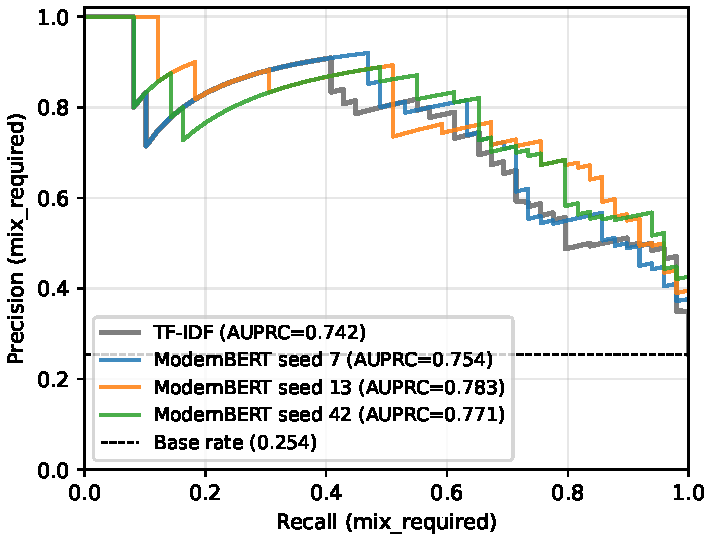
\includegraphics[width=0.85\textwidth]{figures/thesis/pr_curve_test.pdf}
\caption{Precision--recall curves on the held-out test split for the \gls{tfidf} baseline and the three ModernBERT training seeds. The dashed horizontal line is the test-set base rate of \texttt{mix\_required}.}
\label{fig:prCurveTest}
\end{figure}

\begin{figure}[!ht]
\centering
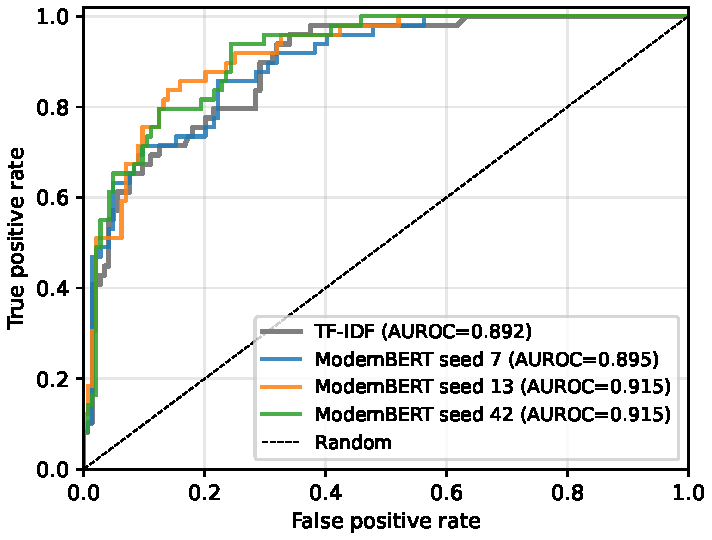
\includegraphics[width=0.85\textwidth]{figures/thesis/roc_curve_test.pdf}
\caption{Receiver-operating-characteristic curves on the held-out test split.}
\label{fig:rocCurveTest}
\end{figure}

Figure~\ref{fig:thresholdVsF1} shows how F1 on \texttt{mix\_required} varies with the decision threshold on the test split, with the validation-selected threshold of each model marked as a dot. The three ModernBERT seeds select different validation thresholds ($\tau^\star = 0.24, 0.36, 0.42$ for seeds $42$, $7$, $13$). Their test F1 at the chosen threshold is consistent across seeds (mean $0.699$, standard deviation $0.017$), which indicates that the F1 plateau is broad and that the choice of operating threshold is not a brittle hyperparameter for these routers.

\begin{figure}[!ht]
\centering
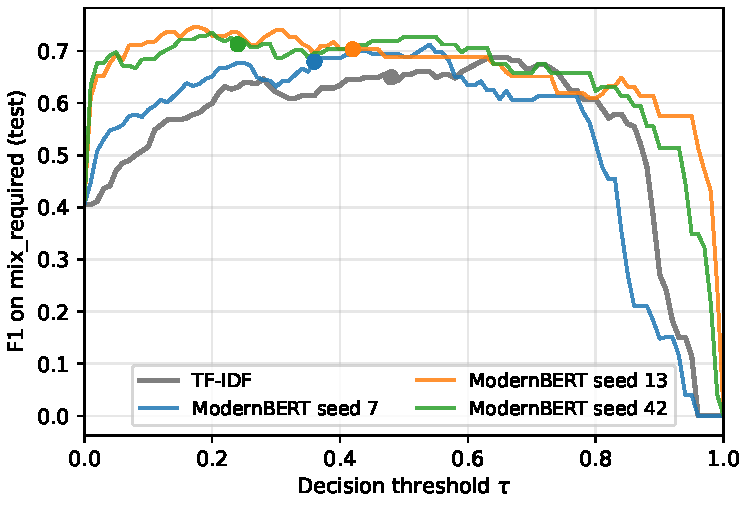
\includegraphics[width=0.85\textwidth]{figures/thesis/threshold_vs_f1_mix.pdf}
\caption{F1 on \texttt{mix\_required} as a function of the decision threshold on the held-out test split. Dots mark the validation-selected threshold for each model: TF-IDF $\tau^\star = 0.48$, ModernBERT seed $42$ $\tau^\star = 0.24$, seed $7$ $\tau^\star = 0.36$, seed $13$ $\tau^\star = 0.42$.}
\label{fig:thresholdVsF1}
\end{figure}

Figure~\ref{fig:thresholdVsTime} shows the mean routed time on test as the threshold sweeps from $0$ (every query routed to \emph{Mix}) to $1$ (every query routed to \emph{Naive}). The always-\emph{Naive} and always-\emph{Mix} levels are shown as horizontal dashed lines and act as a sanity check. At $\tau = 0$ every router collapses to always-\emph{Mix}, and at $\tau = 1$ every router collapses to always-\emph{Naive}, which is what the figure shows.

\begin{figure}[!ht]
\centering
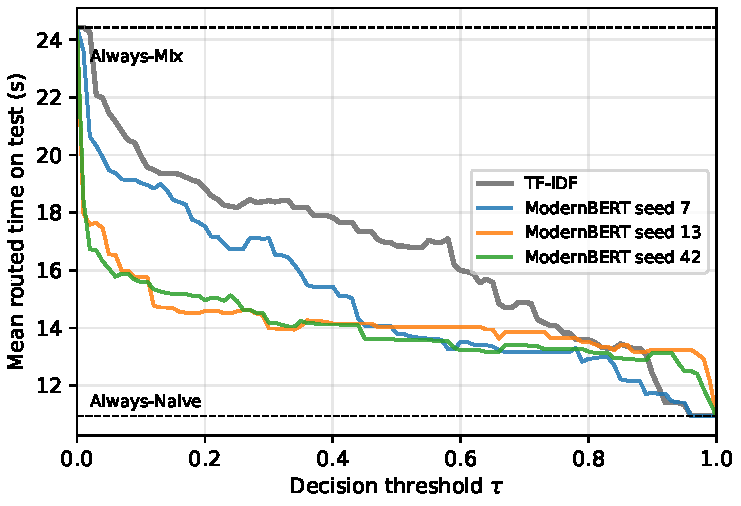
\includegraphics[width=0.85\textwidth]{figures/thesis/threshold_vs_routed_time.pdf}
\caption{Mean routed execution time on the held-out test split as the decision threshold sweeps. The two horizontal dashed lines are the always-\emph{Naive} and always-\emph{Mix} reference levels.}
\label{fig:thresholdVsTime}
\end{figure}

Figure~\ref{fig:costFrontier} combines the two preceding views into a frontier of routing-label F1 against mean routed execution time. Each router traces an operating curve in (mean routed time, F1\textsubscript{mix}) space as $\tau$ sweeps. The static always-\emph{Naive} and always-\emph{Mix} policies appear as the two extreme operating points. Both learned routers achieve higher routing-label F1 than either static policy at substantially lower mean routed time than always-\emph{Mix}. The ModernBERT operating point reaches a higher F1\textsubscript{mix} than \gls{tfidf} at a comparable mean routed time, and the type-only diagnostic baseline sits nearby as a non-deployable reference.

\begin{figure}[!ht]
\centering
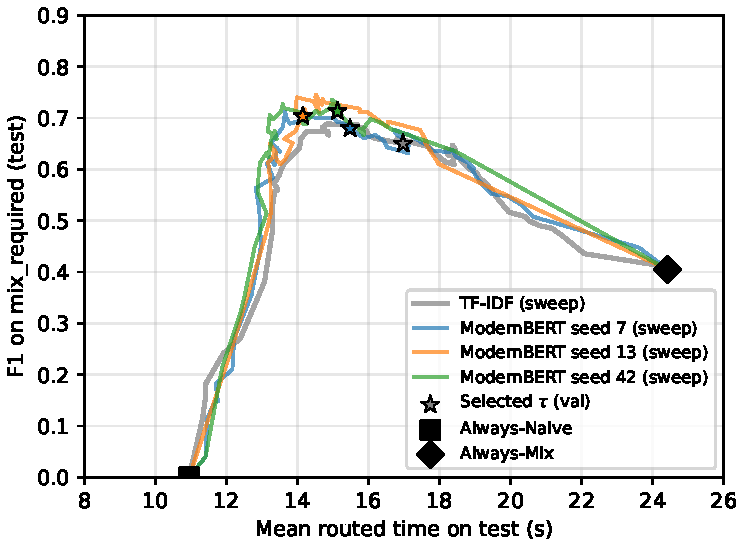
\includegraphics[width=0.85\textwidth]{figures/thesis/cost_performance_frontier.pdf}
\caption{Routing-label F1 on the \texttt{mix\_required} class versus mean routed execution time on the held-out test split. Each curve traces the operating points obtained by sweeping the decision threshold. Stars mark the validation-selected thresholds. Static always-\emph{Naive} and always-\emph{Mix} policies are shown as reference points.}
\label{fig:costFrontier}
\end{figure}

Table~\ref{tab:perQuestionType} reports a per-question-type breakdown on the test split. The four 2WikiMultihopQA question types carry very different fractions of \emph{Mix}-beneficial queries on this split: $2$ out of $90$ for \texttt{comparison}, $8$ out of $33$ for \texttt{bridge\_comparison}, $38$ out of $65$ for \texttt{compositional}, and $1$ out of $5$ for \texttt{inference}. The \texttt{compositional} slice is the one in which the routing decision matters most. The \texttt{inference} slice has too few rows to support stable estimates, so its per-class metrics are reported for completeness only. On \texttt{compositional}, ModernBERT achieves higher point estimates than \gls{tfidf} on both \gls{auprc} (mean $0.839$ vs.\ $0.814$) and F1 on \texttt{mix\_required} (mean $0.799$ vs.\ $0.753$). On \texttt{bridge\_comparison} the two routers trade strengths: \gls{tfidf} routes more queries to \emph{Mix} on this slice and reaches higher recall ($0.375$ vs.\ $0.167$), slightly higher \gls{auprc} ($0.418$ vs.\ $0.363$), and slightly higher F1 ($0.316$ vs.\ $0.211$), while ModernBERT keeps higher precision ($0.345$ vs.\ $0.273$) and higher overall slice accuracy ($0.707$ vs.\ $0.606$).

\begin{table}[!ht]
\centering
\caption{Per-question-type breakdown on the test split. Each row reports the metrics for one 2WikiMultihopQA question type. \emph{Slice} is the question-type label assigned by the benchmark. \emph{n} is the number of test queries in the slice and \emph{n\textsubscript{mix}} is the number of those that are labeled \texttt{mix\_required} by the judge. \emph{Model} is the router whose predictions are scored on the slice. \emph{Acc.}\ is the fraction of slice queries on which the router agrees with the judge-derived routing label. The remaining columns (\gls{auprc}, \emph{P\textsubscript{mix}}, \emph{R\textsubscript{mix}}, \emph{F1\textsubscript{mix}}) carry the same meaning as in Table~\ref{tab:classificationResults} but are computed only from the rows that fall in this slice, with threshold metrics evaluated at each router's validation-selected threshold. The \texttt{comparison} and \texttt{inference} slices contain too few \texttt{mix\_required} positives ($2$ and $1$ respectively) to give informative \gls{auprc} or F1 values, so those entries describe the particular test rows and should not be read as stable estimates. ModernBERT values are the mean over three seeds.}
\label{tab:perQuestionType}
\resizebox{\textwidth}{!}{%
\begin{tabular}{l|rrrrrrrr}
\textbf{Slice} & \textbf{n} & \textbf{n\textsubscript{mix}} & \textbf{Model} & \textbf{AUPRC} & \textbf{P\textsubscript{mix}} & \textbf{R\textsubscript{mix}} & \textbf{F1\textsubscript{mix}} & \textbf{Acc.} \\
\hline
comparison        &  90 &  2 & TF-IDF     & 0.277 & 0.000 & 0.000 & 0.000 & 0.978 \\
                  &     &    & ModernBERT & 0.237 & 0.000 & 0.000 & 0.000 & 0.978 \\
\hline
compositional     &  65 & 38 & TF-IDF     & 0.814 & 0.636 & 0.921 & 0.753 & 0.646 \\
                  &     &    & ModernBERT & 0.839 & 0.741 & 0.868 & 0.799 & 0.744 \\
\hline
bridge\_comparison&  33 &  8 & TF-IDF     & 0.418 & 0.273 & 0.375 & 0.316 & 0.606 \\
                  &     &    & ModernBERT & 0.363 & 0.345 & 0.167 & 0.211 & 0.707 \\
\hline
inference         &   5 &  1 & TF-IDF     & 0.333 & 0.000 & 0.000 & 0.000 & 0.400 \\
                  &     &    & ModernBERT & 0.833 & 0.000 & 0.000 & 0.000 & 0.733 \\
\end{tabular}%
}
\end{table}

Figure~\ref{fig:perQt} visualizes the \gls{auprc} comparison on the two non-degenerate slices.

\begin{figure}[!ht]
\centering
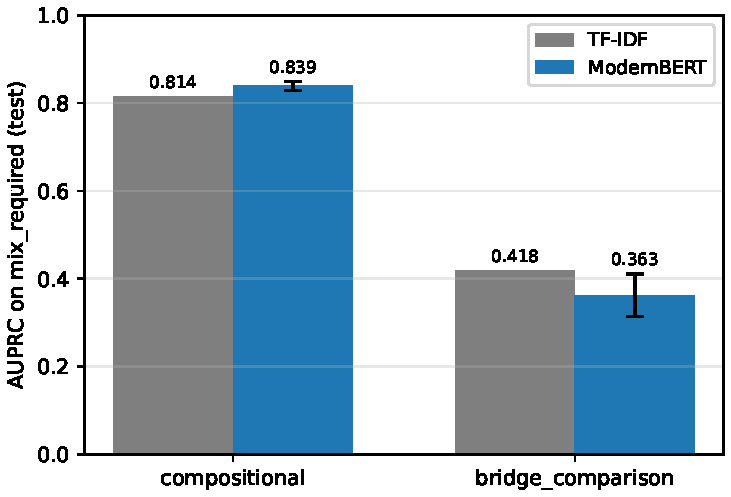
\includegraphics[width=0.85\textwidth]{figures/thesis/per_question_type_auprc.pdf}
\caption{\Gls{auprc} on the \texttt{mix\_required} class, broken down by 2WikiMultihopQA question type on the held-out test split. ModernBERT bars show the mean over three training seeds with error bars at one standard deviation. The \texttt{comparison} and \texttt{inference} slices have too few \texttt{mix\_required} test rows to give an informative \gls{auprc} and are omitted.}
\label{fig:perQt}
\end{figure}

\section{Discussion}
\label{sec:implDiscussion}

The retrieval-mode distinction between \emph{Naive} and \emph{Mix} is partly predictable from the query text alone. Both learned routers outperform the always-\emph{Naive} baseline on the minority class and reach operating points in Figure~\ref{fig:costFrontier} that no static policy at comparable cost can match. The ModernBERT router achieves higher point estimates than \gls{tfidf} on \gls{auprc}, balanced routing-label accuracy, F1 on the minority class, and routing-label accuracy, and these gains are stable across three training seeds.

The two routing error types have different practical weight. A false negative routes a \emph{Mix}-beneficial query to \emph{Naive} and so risks an answer-quality regression on a query where \emph{Mix} was judged necessary. A false positive routes a \emph{Naive}-sufficient query to \emph{Mix} and only wastes compute, because \emph{Naive} was already judged sufficient. This asymmetry explains why always-\emph{Mix} scores poorly on routing-label accuracy without necessarily producing worse final answers, and it also explains the gap between \gls{tfidf} and ModernBERT in Table~\ref{tab:routedCostResults}: \gls{tfidf} has higher recall and lower under-routing, so it misses fewer \emph{Mix}-beneficial queries; ModernBERT has higher precision and lower over-routing, so it issues fewer unnecessary \emph{Mix} calls.

Routing-label performance and routed cost must therefore be interpreted together. The selected ModernBERT operating point behaves selectively, saving more compute at the cost of accepting somewhat more under-routing risk. The \gls{tfidf} operating point behaves conservatively in the opposite direction. Neither extreme is universally correct: which is preferable depends on the relative cost of an unnecessary \emph{Mix} call against an answer-quality regression in a given deployment.

The \texttt{compositional} slice is the most informative one because the class distribution is balanced and \emph{Mix} is judged beneficial on most of its queries. On this slice ModernBERT achieves a mean \gls{auprc} of $0.839$ against $0.814$ for \gls{tfidf} and lifts F1 on \texttt{mix\_required} from $0.753$ to $0.799$. The gain on \texttt{compositional} despite the small training set indicates that the encoder picks up on more than the surface lexical patterns a \gls{tfidf} classifier can exploit. The \texttt{bridge\_comparison} slice is harder for both routers and is the natural target for follow-up work; on this slice \gls{tfidf} reaches a slightly higher \gls{auprc} ($0.418$) and F1 ($0.316$) by routing more queries to \emph{Mix}, while ModernBERT keeps higher precision and higher slice accuracy at the cost of missing more \emph{Mix}-beneficial queries.

The type-only diagnostic baseline shows that a substantial part of the routing signal is already captured by a coarse categorical label about the question. Predicting \emph{Mix} for \texttt{compositional} questions and \emph{Naive} for the rest already reaches an F1 of $0.667$ on Table~\ref{tab:classificationResults}, because \texttt{compositional} questions dominate the \emph{Mix}-beneficial class on this benchmark. The learned router remains useful because such a category label is benchmark metadata and is unavailable in real user deployments. ModernBERT, which sees only the query text, achieves higher point estimates than this categorical rule on F1, precision, and routing-label accuracy.

The router should therefore be understood as predicting an operational label. It picks up patterns in how questions are phrased that correlate with whether \emph{Mix} is judged beneficial under this LightRAG setup and this benchmark distribution. The type-only diagnostic baseline serves as a ceiling on what coarse benchmark structure alone can deliver. Anything ModernBERT adds beyond that ceiling reflects what the encoder learns from phrasing; anything it does not exceed reflects benchmark structure more than a deeper property of the queries.

The per-question-type breakdown and the type-only diagnostic baseline both rely on the benchmark's per-question category label. In a real deployment that label does not exist; users send free-form queries and the routing layer sees only the query text. The category-based slices are useful as a diagnostic device because they show which subpopulations the router handles well and which it does not, and they help separate signal that comes from coarse structural cues (such as whether the question is a compositional multi-hop lookup) from signal that comes from finer phrasing. They are not a deployment recipe; the learned routers approximate the same structure from the query text alone, which is the only input available outside the benchmark.

The same framing helps interpret the contrast between the \texttt{compositional} and \texttt{bridge\_comparison} slices. The fact that ModernBERT is strong on \texttt{compositional} and weaker on \texttt{bridge\_comparison} indicates which phrasings the encoder has learned to recognize on this benchmark, and does not extend to a claim that \texttt{compositional} queries are easier to route in production. Within this benchmark, the \texttt{compositional} slice contains more rows and the rows share a more consistent surface form.

Always-\emph{Mix} illustrates why the two result tables must be read together. It is label-incorrect on \emph{Naive}-sufficient rows because it uses more retrieval than necessary, although the underlying \emph{Mix} answer on those rows can still be correct. The absence of a direct final-answer-accuracy comparison for each routed policy is treated as a limitation in Section~\ref{sec:limitFinalAnswerAccuracy}.

The reported metrics are still informative for adaptive routing. Routing-label F1 measures whether the router selects the minimum judged sufficient mode. Mean routed time and estimated token usage measure the cost of doing so. The under-routing and over-routing rates separate answer-risk errors from cost-waste errors. Together they describe how often the router agrees with the judge and how expensive that agreement is.

The held-out test set has $193$ queries. This is large enough to compute meaningful bootstrap intervals and too small to resolve small differences between the routers with confidence. The \gls{tfidf} bootstrap \gls{auroc} interval ($[0.836, 0.936]$) contains the ModernBERT mean \gls{auroc} of $0.908$, so the \gls{auroc} comparison is not significant on this test set. The \gls{auprc} and balanced-routing-label-accuracy gaps are larger and still lie inside the bootstrap intervals, as expected on a $193$-row test set. The multi-seed standard deviation for ModernBERT is small on the aggregate routing-label metrics ($\leq 0.017$ on \gls{auprc}, \gls{auroc}, balanced routing-label accuracy, F1, and routing-label accuracy), so the gains are at least stable across seeds. Per-class precision and recall vary more across seeds (standard deviations of $0.057$ and $0.042$), which is what one would expect when each seed selects its own decision threshold on a $193$-row test set. A larger benchmark would be needed before stronger claims can be made.

Finally, the cost picture is sharper in model tokens than in execution time. The two static baselines bracket a mean routed range of $10.95$ to $24.42$ seconds per query in execution time, and $3{,}458$ to $17{,}857$ tokens per query in model-token usage. The learned routers select operating points around $15$ to $17$ seconds per query (a $30$--$39\,\%$ reduction relative to always-\emph{Mix}) and $7{,}100$ to $8{,}500$ tokens per query (a $52$--$60\,\%$ reduction relative to always-\emph{Mix}), at non-trivial \texttt{mix\_required} F1. Tokens move further than time because \emph{Mix} adds one extra LLM call per query and a substantially larger assembled context \cite{lightrag2024,microsoft2024graphragcosts}, while execution time is partly absorbed by network latency that does not scale with token volume. The routing decision itself contributes essentially zero LLM tokens because neither router calls a generative model, and only milliseconds of compute time, which is negligible against retrieval cost on either dimension.

\cleardoublepage
\chapter{Conclusions and future work}
\label{ch:conclusionsAndFutureWork}

This chapter summarizes the conclusions from the experiments (Section~\ref{sec:conclusions}), discusses the main limitations and natural avenues for future work (Section~\ref{sec:limitationsFutureWork}), and reflects on the broader context of the project (Section~\ref{sec:reflections}).

\section{Conclusions}
\label{sec:conclusions}

This thesis studied whether the choice between LightRAG's cheap \emph{Naive} retrieval mode and its more expensive \emph{Mix} retrieval mode can be predicted from the query text alone, on the 2WikiMultihopQA benchmark, using a lightweight encoder-only classifier instead of a large language-model controller. Routing labels were derived by running both retrieval modes on each benchmark question and asking an \gls{llmjudge} \cite{zheng2023judge} to compare each mode's answer against the gold answer. The label \texttt{mix\_required} is operational: it captures whether \emph{Mix} was judged correct when \emph{Naive} was not under the chosen LightRAG configuration and judge prompt, and it does not isolate which component of \emph{Mix} drove the improvement.

The research question asks, within a fixed Hybrid \gls{rag} setting, how well a lightweight query-only classifier predicts a judge-derived routing label for the minimum sufficient retrieval mode, and how using that classifier as an offline routing policy affects routed cost relative to static \emph{Naive} and \emph{Mix} baselines. The remainder of this section answers the three sub-questions in turn.

The first sub-question concerns classifier accuracy on the routing label. On the held-out test split of $193$ queries, the ModernBERT router achieves higher point estimates than the \gls{tfidf} baseline on every aggregate routing-label metric: \gls{auprc} ($0.769$ vs.\ $0.742$), balanced routing-label accuracy ($0.798$ vs.\ $0.784$), F1 on the minority \texttt{mix\_required} class ($0.699$ vs.\ $0.650$), and routing-label accuracy ($0.846$ vs.\ $0.788$). The \gls{auroc} gap is inside the bootstrap interval and is therefore not significant. The multi-seed standard deviation of the ModernBERT router is small on the aggregate routing-label metrics ($\leq 0.017$ on \gls{auprc}, \gls{auroc}, balanced routing-label accuracy, F1, and routing-label accuracy), which indicates that the gains are stable across initialization seeds. The two routers also place themselves at opposite ends of the precision-recall trade-off on the \texttt{mix\_required} class: \gls{tfidf} has lower under-routing ($0.057$ vs.\ $0.076 \pm 0.009$), and ModernBERT has lower over-routing ($0.078 \pm 0.019$ vs.\ $0.155$).

The second sub-question concerns routed cost relative to static baselines. Both learned routers reach test-set operating points around $15$ to $17$ seconds of mean routed execution time, compared with $10.95$ seconds for always-\emph{Naive} and $24.42$ seconds for always-\emph{Mix}, and achieve higher routing-label F1 than either static policy at substantially lower mean routed time than always-\emph{Mix}. Measured in model tokens, they route at roughly $7{,}100$ to $8{,}500$ tokens per query, compared with $3{,}458$ for always-\emph{Naive} and $17{,}857$ for always-\emph{Mix}. The selected ModernBERT operating point reduces estimated routed token cost by $60\,\%$ relative to always-\emph{Mix}, and the selected \gls{tfidf} operating point by $52\,\%$. The routing decision itself adds negligible cost on either dimension because neither router calls a generative model.

The third sub-question asks how much a query-only learned router improves over a heuristic that routes by a coarse question-category label alone. The type-only diagnostic baseline, which predicts \emph{Mix} for \texttt{compositional} questions and \emph{Naive} otherwise, already reaches an F1 of $0.667$, a balanced routing-label accuracy of $0.794$, and a routing-label accuracy of $0.803$ on the test split. ModernBERT, which sees only the query text and never the category label, improves on this categorical rule on F1, precision, and routing-label accuracy. The categorical rule is not a realistic deployment policy because such a label is not generally available for arbitrary user queries, while a query-only router needs only the query text. Most of the remaining signal localizes in the \texttt{compositional} slice, where ModernBERT achieves a roughly two-and-a-half-point higher \gls{auprc} than \gls{tfidf}. The \texttt{bridge\_comparison} slice is the weakest part of the result and is a natural target for further work.

Taken together, the three answers indicate that the \emph{Naive}-sufficient versus \emph{Mix}-beneficial distinction is partly predictable from query text alone in this setting, and that a lightweight encoder classifier extracts more of that predictability than a \gls{tfidf} logistic-regression baseline or a coarse question-category heuristic. The reported accuracy values are routing-label accuracies, and they are distinct from independently measured final answer accuracies. Within that scope, the result supports learned query routing as a promising cost-control layer for Hybrid \gls{rag}: the router can often identify when the expensive path is unnecessary, and it therefore reduces routed cost without always defaulting to the most expensive retrieval mode.

\section{Limitations and future work}
\label{sec:limitationsFutureWork}

\subsection{Token-cost measurement scope}
\label{sec:limitTokenCost}

Model-token cost in this thesis is estimated using per-mode mean token usage from an instrumented subset of \(N = 150\) queries spanning all four 2WikiMultihopQA question types. This subset is large enough to give a stable per-mode mean, and it is still smaller than the full $1{,}286$-row routing dataset. The reported token costs should therefore be read as estimated routed token usage from per-mode means, and not as exact measured token usage for every held-out query.

Future work should log token usage for every \emph{Naive} and \emph{Mix} execution in the full $1{,}286$-row routing dataset. With per-query token logging it becomes possible to compute per-query routed token cost directly, to report bootstrap intervals for token cost on the same footing as for execution time, and to study whether token usage varies systematically across question types or routing labels.

\subsection{Judge labels}
\label{sec:limitJudgeLabels}

Routing labels come from an \gls{llmjudge} and are used as judged supervision, not as absolute ground truth. The judge sees the gold answer and the same prompt is used consistently across the dataset \cite{zheng2023judge}, but judge errors may still propagate into the labels. The risk is largest for borderline answers, partially correct answers, and answers that use different surface forms from the gold answer.

The label \texttt{mix\_required} should be read operationally: it captures cases in which \emph{Mix} was judged correct when \emph{Naive} was not under the chosen LightRAG configuration and judge prompt, and it does not isolate which component of \emph{Mix} caused the improvement. \emph{Mix} differs from \emph{Naive} in graph traversal, context assembly, and retrieval breadth, and the label aggregates over all of these.

Useful follow-up work includes validating a sample of judge decisions manually, comparing multiple judge models, and tightening the answer-normalization rules where possible.

\subsection{Final answer accuracy of routed policies}
\label{sec:limitFinalAnswerAccuracy}

The offline policy evaluation reports routing-label performance and routed cost. It does not independently re-judge the final answer selected by each routed policy. This matters because false-positive \emph{Mix} decisions are counted as routing-label errors, although the \emph{Mix} answer for the same query may still be correct. False-negative \emph{Mix} decisions are the errors most directly associated with answer-quality risk, because the router selects \emph{Naive} on a query where \emph{Mix} was judged necessary.

A future evaluation should retain per-mode correctness indicators for every query, or re-run the judge on the answer selected by each policy, so that judged final answer accuracy can be reported alongside routed cost. With per-policy answer correctness available, the main trade-off would become answer correctness against token cost.

\subsection{Generalizability}
\label{sec:limitGeneralizability}

The experiments use one Hybrid \gls{rag} framework (LightRAG), two of its retrieval modes (\emph{Naive} and \emph{Mix}), and one public benchmark (2WikiMultihopQA). The held-out test set has $193$ rows, which is enough to compute bootstrap intervals and not enough to resolve small differences between routers. The conclusions therefore apply most directly to the studied setting. Applying the same methodology to other Hybrid \gls{rag} frameworks (for example GraphRAG \cite{edge2024graphrag} or hybrid retrieval modes in other systems) and to other multi-hop benchmarks (HotpotQA, MuSiQue \cite{yang2018hotpotqa,trivedi2022musique}) is a natural way to test how robust the routing signal is. Extending the routing labels to industrial corpora (for example Ericsson internal documentation) was considered but is blocked by the absence of per-query gold answers, which is what made the judge-labeling protocol possible on 2WikiMultihopQA in the first place.

The strong type-only diagnostic baseline also indicates that part of the routing signal may be benchmark-specific. The results should not be read as evidence that the same router would transfer unchanged to arbitrary industrial queries without additional validation.

\subsection{Routing beyond the query}
\label{sec:limitRouting}

The router used in this thesis is query-only by construction. A router that also has access to some lightweight signal from the corpus or from a cheap first retrieval pass could in principle make a better decision, at the cost of a slightly more expensive routing layer. A natural follow-up is to compare the query-only router against a two-stage scheme that first runs the cheap \emph{Naive} mode, inspects whether the retrieved chunks contain the entities referenced in the query, and escalates to \emph{Mix} only when this signal looks weak. This is similar to how Adaptive-RAG conditions on cheap intermediate signals at the language-model level \cite{jeong2024adaptiverag}. The routing layer would still be cheap (one round of vector retrieval instead of an expensive graph traversal) and could materially improve the harder slices, in particular \texttt{bridge\_comparison}.

\subsection{Calibration and abstention}
\label{sec:limitCalibration}

The router currently outputs a single thresholded decision. Routing under cost constraints is a natural setting for selective prediction \cite{geifman2017selective} and calibrated probabilities \cite{guo2017calibration}, where the router could abstain on low-confidence queries and either escalate to a more expensive but more reliable controller or run both retrieval modes and combine the answers. The calibration of the ModernBERT router's softmax outputs was not investigated in this work and is a natural follow-up.

\section{Reflections}
\label{sec:reflections}

This thesis is centered on making a Hybrid \gls{rag} system more resource-efficient. The most direct connection is to the \gls{UN} \gls{SDG} number 12 (responsible consumption and production). Graph-enhanced retrieval is significantly more compute-intensive than vector retrieval \cite{lightrag2024,microsoft2024graphragcosts}, and a router that avoids applying it to queries that do not need it directly reduces the energy and compute footprint of the system at inference time. There is also a softer connection to \gls{SDG} number 9 (industry, innovation, and infrastructure), in that adaptive routing is a building block for industrial \gls{rag} deployments such as the one motivating this work at Ericsson, where serving company-internal documentation at scale is a real operational concern.

The work has some ethical aspects worth flagging. The routing labels are produced by an \gls{llmjudge} that has access to the gold answer. This is a methodologically reasonable but imperfect protocol, and the thesis is explicit about not treating these labels as ground truth. Building a system that decides on a per-query basis which retrieval path to use could in principle interact with downstream notions of answer quality in ways that are hard to anticipate. If the router systematically routes some kind of question to the cheaper path, that kind of question could end up consistently worse-served, even when the average behavior of the system improves. The per-question-type breakdown in Section~\ref{sec:implResults} is one way to surface this kind of differential behavior, and any future work that scales this approach to user-facing settings should keep similar per-segment analyses in view.

\noindent\rule{\textwidth}{0.4mm}

\cleardoublepage
% Print the bibliography (and make it appear in the table of contents)
\renewcommand{\bibname}{References}


\iftoggle{biblatex}{
    %\typeout{Biblatex current language is \currentlang}
    \printbibliography[heading=bibintoc]
}{
    \phantomsection  % make it include a hyperref - see https://tex.stackexchange.com/a/98995
    \addcontentsline{toc}{chapter}{References}
    \bibliography{references}
}



\cleardoublepage
\appendix
\renewcommand{\chaptermark}[1]{\markboth{Appendix \thechapter\relax:\thinspace\relax#1}{}}
\chapter{Source code}
\label{sec:supportingMaterial}

The implementation code, the data-preparation pipeline, the training scripts, and the evaluation scripts used in this thesis are publicly available at \url{\thesisCodeUrl}.

\cleardoublepage

\chapter{Experimental configuration}
\label{app:experimentalConfig}

This appendix lists the configuration used to produce the routing labels, train the routers, and compute the reported routed-cost estimates. Table~\ref{tab:lightragDataJudgeConfig} summarizes the LightRAG, data, and judge settings. Table~\ref{tab:routerTrainingConfig} summarizes the router training settings. Section~\ref{app:pipelineScripts} maps each pipeline stage onto a script in the public code repository (Appendix~\ref{sec:supportingMaterial}), and Section~\ref{app:judgePrompt} reproduces the judge prompt verbatim.

\begin{table}[!ht]
\centering
\caption{LightRAG, data, and judge configuration used in this thesis. Each row names one configurable component of the pipeline and gives the exact value used in all reported experiments. \emph{Item} is the name of the component (model checkpoint, framework version, retrieval parameter, or instrumentation choice); \emph{Value} is the literal value passed to the corresponding API or library. The same generator model and embedding model are used during indexing and at query time. All Gemini calls use a temperature of $0.0$.}
\label{tab:lightragDataJudgeConfig}
\begin{tabularx}{\textwidth}{p{0.34\textwidth}|X}
\textbf{Item} & \textbf{Value} \\
\hline
Generator model & \texttt{gemini-3-flash-preview} (Gemini API) \\
Judge model & \texttt{gemini-3-flash-preview} (Gemini API) \\
Embedding model & \texttt{models/gemini-embedding-001} (768-dim) \\
LightRAG version & \texttt{1.4.10} (vendored fork in \texttt{external/LightRAG}) \\
LightRAG chunk token size & 1\,200 tokens \\
LightRAG chunk overlap & 100 tokens \\
\emph{Naive} retrieval parameters & \texttt{top\_k=3}, \texttt{chunk\_top\_k=3} \\
\emph{Mix} retrieval parameters & \texttt{mode="mix"}, \texttt{chunk\_top\_k=3}; entity-relation graph built during indexing \\
LightRAG tokenizer & \texttt{gpt-4o-mini} via \texttt{tiktoken} \\
Generator temperature & 0.0 \\
Judge temperature & 0.0 \\
Token logging method & Gemini API \texttt{usage\_metadata} per LLM call, plus tiktoken estimates for embedding calls when the API does not report tokens \\
Token measurement subset & \(N = 150\) queries spanning all four 2WikiMultihopQA question types \\
Judge prompt location & Section~\ref{app:judgePrompt} \\
\end{tabularx}
\end{table}

\begin{table}[!ht]
\centering
\caption{Router training configuration used in this thesis. Each row names one router hyperparameter or training-pipeline setting and gives the exact value used in all reported experiments. \emph{Item} is the name of the hyperparameter or setting; \emph{Value} is the value passed to scikit-learn (for the \gls{tfidf} baseline) or Hugging Face Transformers (for the ModernBERT router). All three ModernBERT seeds use the values listed here; only the random seed differs across the three runs.}
\label{tab:routerTrainingConfig}
\begin{tabularx}{\textwidth}{p{0.34\textwidth}|X}
\textbf{Item} & \textbf{Value} \\
\hline
TF-IDF features & Unigrams and bigrams, lowercase, English stop-words removed, min document frequency 2, vocabulary cap 20\,000 \\
TF-IDF classifier & Logistic regression, $L_2$ regularization with $C=1.0$, balanced class weights, scikit-learn L-BFGS solver, max 1\,000 iterations \\
ModernBERT checkpoint & \texttt{answerdotai/ModernBERT-base} \\
ModernBERT max sequence length & 128 tokens \\
ModernBERT learning rate & $2 \times 10^{-5}$ \\
ModernBERT weight decay & 0.01 \\
ModernBERT batch size & Per-device $8$, gradient accumulation $2$, effective batch $16$ \\
ModernBERT optimizer & AdamW with linear warm-up over $10\,\%$ of steps and linear decay; gradient clip $1.0$ \\
ModernBERT max epochs & 8, early stopping on validation F1\textsubscript{mix} with patience 3, minimum 3 epochs \\
ModernBERT seeds & 7, 13, 42 \\
Split sizes & 900 train / 193 validation / 193 test \\
Split strategy & Joint stratification by question type and routing label \\
Hardware & Single CPU; no GPU used for ModernBERT training or inference \\
\end{tabularx}
\end{table}

\section{Pipeline scripts}
\label{app:pipelineScripts}

The eight pipeline stages used in this thesis map one-to-one onto scripts in the public code repository (Appendix~\ref{sec:supportingMaterial}). Table~\ref{tab:pipelineScripts} lists the script for each stage in the order it is executed. Running the scripts in this order reproduces the data, the routers, and the figures used in this thesis from the raw 2WikiMultihopQA download.

\begin{table}[!ht]
\centering
\caption{Pipeline stages and the script that implements each stage. \emph{Stage} names a logical step of the data and modelling pipeline (sample preparation, indexing, dual-mode execution, token instrumentation, judging, dataset construction, router training, evaluation, or figure generation). \emph{Script} is the path of the Python file in the public code repository (Appendix~\ref{sec:supportingMaterial}) that implements the stage; all paths are relative to the repository root. Running the scripts in the order shown reproduces the data, routers, and figures used in this thesis from the raw 2WikiMultihopQA download.}
\label{tab:pipelineScripts}
\begin{tabularx}{\textwidth}{p{0.36\textwidth}|X}
\textbf{Stage} & \textbf{Script} \\
\hline
Prepare 2WikiMultihopQA samples & \texttt{src/dataset\_tools/prepare\_2wiki\_samples.py} \\
Index the corpus in LightRAG & \texttt{src/data\_synthesis/index\_2wiki\_lightrag.py} \\
Run both retrieval modes on every queryable sample & \texttt{src/data\_synthesis/query\_lightrag.py} \\
Instrument token usage on the \(N = 150\) subset & \texttt{src/data\_synthesis/query\_lightrag\_token\_usage.py} \\
Generate routing labels with LLM-as-a-Judge & \texttt{src/data\_synthesis/judge\_query\_results.py} \\
Build the binary routing dataset and joint-stratified splits & \texttt{src/router/prepare\_router\_dataset.py} \\
Train the TF-IDF baseline router & \texttt{src/router/train\_baseline\_router.py} \\
Train the ModernBERT routers (seeds 7, 13, 42) & \texttt{src/router/train\_modernbert\_router.py} \\
Run held-out classification, routed-cost simulation, per-question-type breakdown, bootstrap CIs, multi-seed aggregation & \texttt{src/router/thesis\_analysis.py} \\
Generate the figures used in this thesis & \texttt{src/router/thesis\_figures.py} \\
\end{tabularx}
\end{table}

\section{Judge prompt}
\label{app:judgePrompt}

The judge receives the question, the gold answer, the \emph{Naive} answer, and the \emph{Mix} answer in a JSON payload, and is asked to return exactly one of the three class labels \texttt{naive\_enough}, \texttt{mix\_required}, or \texttt{none\_enough}. The system prompt is reproduced verbatim below; the label semantics that the judge enforces are added below the verbatim prompt as inline annotations and are not part of the prompt itself.

\begin{lstlisting}[basicstyle=\ttfamily\small,breaklines=true,columns=fullflexible]
You are a strict evaluator for a retrieval-routing dataset.
You must output exactly one class label and nothing else.
Allowed labels:
- naive_enough
- mix_required
- none_enough

# Label semantics (annotation, not part of the prompt):
# naive_enough  -> the Naive answer matches the gold answer
# mix_required  -> the Naive answer does not match the gold answer
#                  but the Mix answer does
# none_enough   -> neither answer matches the gold answer;
#                  these rows are excluded from the binary routing dataset
\end{lstlisting}

\cleardoublepage

\begin{comment}
% If you actually want to have the full table of National Subject Categories (temporarily) include this appendix
\subfile{README_notes/National_Subject_Categories}
\cleardoublepage
\end{comment}

\begin{comment}
% Information for examiners
\ifxeorlua
\cleardoublepage
\input{README_notes/README_examiner_notes}
\fi
\end{comment}

\begin{comment}
% Information for administrators
\ifxeorlua
\cleardoublepage
\input{README_notes/README_for_administrators.tex}
\fi
\end{comment}

\begin{comment}
% Information for Course Coordinators
\ifxeorlua
\cleardoublepage
\input{README_notes/README_for_course_coordinators}
\fi
\end{comment}

%% The following label is necessary for computing the last page number of the body of the report to include in the "For DIVA" information
\label{pg:lastPageofMainmatter}

\cleardoublepage
\clearpage\thispagestyle{empty}\mbox{} % empty page with backcover on the other side
\kthbackcover

\end{document}
